\documentclass[conference]{IEEEtran}
\IEEEoverridecommandlockouts
\usepackage{cite}
\usepackage{amsmath,amssymb,amsfonts}
\usepackage{algorithmic}
\usepackage{graphicx}
\usepackage{textcomp}
\usepackage{xcolor}
\usepackage{caption}
\usepackage{subcaption}
\usepackage{algorithm}
\usepackage{algorithmic}
\usepackage{todonotes}

\def\BibTeX{{\rm B\kern-.05em{\sc i\kern-.025em b}\kern-.08em
    T\kern-.1667em\lower.7ex\hbox{E}\kern-.125emX}}
\usepackage{bm}
\begin{document}

\title{Parallel Approximations of the Tukey $g$-and-$h$  Likelihoods and Predictions for Non-Gaussian Geostatistics}




\maketitle

\begin{abstract}

Maximum likelihood estimation is an essential tool in
the procedure to impute missing data in climate/weather
applications. However, its computation demands operations
on a dense symmetric positive definite matrix, parameterized by
the Mat\'ern correlation function. This computation of the log-likelihood requires $\mathcal{O}(n^2)$ storage 
and $\mathcal{O}(n^3)$ operations, which can be a 
huge task considering that the number of geographical 
locations $n$ can be enormous for some problems.  
By defining a particular statistical model, the maximum likelihood estimation can be used to understand the underlying
structure of given geospatial data. The Gaussian random field 
is one of the most popular models that has been widely used 
to describe geospatial data under the hood of maximum likelihood estimation. However, despite its appealing theoretical properties, the assumptions of Gaussianity are unrealistic since real data usually
show signs of skewness or have some extreme values. Herein, we consider the Tukey $g$-and-$h$ (TGH) random field as an example
of a non-Gaussian random field that shows more robustness in modeling geospatial data by including two more parameters 
to incorporate skewness and heavy tail features in the model. 
This work provides the first HPC implementation of the TGH 
random field's inference on parallel hardware architectures. 
Using task-based programming models associated with dynamic runtime systems,
our implementation leverages high concurrency of current parallel systems.
This permits to run the exact log-likelihood evaluation of the Tukey $g$-and-$h$ (TGH) random fields 
for a decent number of geospatial locations.
To tackle large-scale problems, we provide additionally an implementation of the given model 
using two different low-rank approximations. We compress the aforementioned positive-definite symmetric matrix for computing the 
log-likelihood and rely on the Tile Low-Rank (TLR) and the Hierarchical off-Diagonal Low-Rank (HODLR) matrix
approximations. We assess the performance and accuracy of the proposed implementations using synthetic 
datasets up to $800K$ and a $300K$ precipitation data of Germany to demonstrate the advantage 
of using non-Gaussian over Gaussian random fields. Moreover, by relying on TLR/HODLR matrix computations, we 
can now solve for larger matrix sizes, while preserving the required accuracy for prediction. We show
the performance superiority of TLR over HODLR matrix computations when calculating the TGH 
likelihoods and predictions. Our TLR-based approximation shows a 
speedup up to $7.29X$ and $2.96X$ on shared-memory and distributed-memory systems, respectively, compared
to the exact implementation. % while preserving the required accuracy.
\end{abstract}

\section{Introduction}



Techniques relying on latent Gaussian models are widely used to make spatial predictions beyond the observed geographical locations. The target modeling
process involves obtaining a set of statistical parameters
with the aid of the likelihood function through  the Maximum Likelihood Estimation (MLE) method in order to impute missing spatial data.  MLE 
operates on a dense covariance matrix with dimension $n \times n$ where $n$ represents the number of geospatial locations. The challenge for high-dimensional problems lies in the
computation requirements of the log-likelihood function, which necessitates $O(n^3)$ computation and $O(n^2)$ memory space, making its computation prohibitive for large $n$. Techniques exist to tailor  the modeling process to reduce the	 computing cost by order of magnitude. Low-rank approximation has been shown to be necessary for the
closely related problem of the spatial statistics framework~\cite{cressie2008fixed, eidsvik2012approximate, stein2013stochastic, abdulah2018parallel}. However, most of the existing  studies evaluate the effectiveness of the low-rank approximation with the Gaussian process, which is limited in real-life datasets.

In typical applications, the spatial variables are non-Gaussian, where skewness
and heavy tails are captured. A common approach 
to deal with this non-Gaussian behavior is to apply a  non-linear transformation such as 
square-root transform~\cite{berrocal2010bivariate,yao2015fault,yan2019non}, Box–Cox transform ~\cite{de1997bayesian} and the log-normal 
transform~\cite{rios2018learning} which is known as the trans-Gaussian approach. Ideally, transforming non-Gaussian 
data using one of these techniques should be 
enough to apply Gaussian modeling directly to the data. However, it is impossible to find a suitable transformation technique 
that can give the best modeling performance for arbitrary datasets, and some non-Gaussian properties can be lost through the transformation 
process. In~\cite{xu2017tukey}, a highly flexible trans-Gaussian model has been proposed under the name Tukey $g$-and-$h$ (TGH) random
fields.This model is parameterized to capture the non-Gaussianity  through the covariance function estimation and allows better modeling of the underlying geospatial data.

This work presents a parallel implementation of the 
TGH non-Gaussian random fields in the context of climate and environmental applications.
We rely on a task-based programming model to provide
the TGH modeling and prediction operations in the exact form where the dense linear algebra operations have been drawn from 
the Chameleon library~\cite{agullo2017achieving}
and the underlying tasks schedule managed by the StarPU 
runtime system~\cite{augonnet2011starpu}. We also provide two low-rank implementations 
of the TGH model: TLR-based, where the compression and linear algebra operations run through the HiCMA library~\cite{hicma-soft}, and 
Hierarchical off-Diagonal Low-Rank (HODLR)-based approximations~\cite{hodlr-soft}, where the 
compression and linear algebra operations run through HODLRLIB~\cite{hodlr-soft, ambikasaran2013mathcal}.
The TLR-based implementation shows a 
speedup up to $7.29X$ and $2.96X$ on shared-memory and distributed-memory systems, respectively, compared
to exact implementation.

Our main contributions are as follows: 1) We propose a 
parallel implementation of the TGH non-Gaussian likelihoods and predictions to model a wide range of real spatial 
datasets on shared-memory and distributed-memory systems; 2) We provide parallel TLR-based and HODLR-based approximations to the exact predictive model to reduce the 
prohibitive complexity of the underlying algebra operations of the associated dense covariance matrix; 3) We show the effectiveness 
of the non-Gaussian scheme provided by our implementation compared with the traditional Gaussian modeling with both synthetic and real datasets; 4) We provide a comparison in the parameters' estimation accuracy to 
produce  the required accuracy  for both  TLR-based  and HODLR-based approximation; 5) We assess the performance of exact/TLR/HODLR non-Gaussian 
modeling and prediction on shared-memory and distributed-memory systems; and 6) We demonstrate the quality of our 
implementation in a $300K$ precipitation dataset of Germany to show that we are 
able to provide a robust predictive model to work in such a non-Gaussian dataset.


The remainder of the paper is organized as follows. 
Section II covers related work. Section III gives an overview and background of our problem. Section IV describes in detail 
the algorithm and our parallel implementation. Section V analyzes accuracy and performance using synthetic and real
datasets in the context of climate/weather applications. 
We conclude in Section VI.

\section{Related Work} 
%Non-Gaussianit 
%Xu and Genton \cite{2017.G.X.M.G.G.JournaloftheAmericanStatisticalAssociation} introduced the Tukey $g$-and-$h$ random fields to model non-Gaussian geostatistical data. There also exist various kinds of non-Gaussian spatial models in the literature. The Tukey random fields are not the only non-Gaussian Random fields. There exist various kinds of non-Gaussian spatial models in the literature. There exist various kinds of non-Gaussian spatial models. For example, non-Gaussian models based on skew-Gaussian distributions proposed by Kim and Mallick \cite{2004.H.M.K.B.M.JournalofStatisticalPlanningandInference}, Zhang and El-Shaarawi \cite{2010.H.Z.A.E.Environmetrics}, Genton and Zhang \cite{2012.M.G.H.Z.ChileanJournalofStatistics}, Rimstad and Omre \cite{2014.K.R.H.O.SpatialStatistics}, and more recently model based on the skew-$t$ distribution by Bevilacqua et al. \cite{2021.M.B.C.C.R.B.A.V.V.M.ScandinavianJournalofStatistics}; scale mixture of Gaussian random field proposed by Palacios and Steel \cite{2006.M.B.P.M.F.J.S.JournaloftheAmericanStatisticalAssociation} and Fonseca and Steel \cite{2011.T.C.O.F.M.F.J.S.Biometrika}; log-skew-elliptical random fields by Marchenko and Genton \cite{2010.Y.V.M.M.G.Environmetrics}; $T$-distributed random fields by Røislien and Omre \cite{2006.J.R.H.O.MathematicalGeology}; transGaussian random fields by Cressie \cite{1993.N.C.Wiley.Interscience} and by De Oliveira et al. \cite{1997.V.D.O.B.K.D.A.S.JournaloftheAmericanStatisticalAssociation}, by Allcroft and Glasbey \cite{2003.D.J.A.C.A.G.JournaloftheRoyalStatisticalSociety}, and by Butler and Glasbey \cite{2008.A.B.C.A.G.JournaloftheRoyalStatisticalSociety}; spatial copula models by Gräler \cite{2014.B.G.SpatialStatistics} and by Krupskii et al. \cite{2018.P.K.R.H.M.G.G.JournaloftheAmericanStatisticalAssociation} and non-Gaussian Matérn fields by Wallin and Bolin \cite{2015.J.W.D.B.ScandinavianJournalofStatistics}. We use the Tukey random field because of its parsimonious parameterization, its flexible marginal distributions, tractable forms of its log-likelihood, and its prediction function. 
%
%=======

In this section, we discuss some of the popular 
approaches for constructing non-Gaussian random fields. Use of various non-Gaussian distributions such as skew-Gaussian distribution (Kim and Mallick \cite{2004.H.M.K.B.M.JournalofStatisticalPlanningandInference}; Zhang and El-Shaarawi \cite{2010.H.Z.A.E.Environmetrics}; Genton and Zhang \cite{2012.M.G.H.Z.ChileanJournalofStatistics}, Rimstad and Omre \cite{2014.K.R.H.O.SpatialStatistics}), $t$-distribution (Røislien and Omre \cite{2006.J.R.H.O.MathematicalGeology}), 
skew-$t$ distribution (Bevilacqua et al. \cite{2021.M.B.C.C.R.B.A.V.V.M.ScandinavianJournalofStatistics}), log-skew-elliptical distribution (Marchenko and Genton \cite{2010.Y.V.M.M.G.Environmetrics}) can create 
different non-Gaussian random fields. Palacios and Steel \cite{2006.M.B.P.M.F.J.S.JournaloftheAmericanStatisticalAssociation} and Fonseca and Steel \cite{2011.T.C.O.F.M.F.J.S.Biometrika} provided non-Gaussian models for spatial data by scale mixing the Gaussian 
random field. Gräler \cite{2014.B.G.SpatialStatistics} 
and Krupskii et al. \cite{2018.P.K.R.H.M.G.G.JournaloftheAmericanStatisticalAssociation} made non-Gaussian random fields using copula. Wallin and Bolin \cite{2015.J.W.D.B.ScandinavianJournalofStatistics} provided 
a class of non-Gaussian spatial Mat\'ern fields using stochastic partial differential equations. Another popular technique to model 
non-Gaussian spatial data, known as trans-Gaussian 
random field, is applying a non-linear transformation of 
the original data such that the transformed data become Gaussian. 
A few well-used non-linear conversions are log-normal (De Oliveira \cite{2006.V.D.O.ScandinavianJournalofStatistics}), 
square-root (Johns et al. \cite{2003.C.J.J.D.N.T.G.F.K.C.D.JournaloftheAmericanStatisticalAssociation}), Box-Cox (De Oliveira et al. \cite{1997.V.D.O.B.K.D.A.S.JournaloftheAmericanStatisticalAssociation}), and power transformations (Allcroft and Glasbey \cite{2003.D.J.A.C.A.G.JournaloftheRoyalStatisticalSociety}).
 However, it may be  challenging to find this transformation in some situations, if not impossible. Xu and Genton \cite{xu2017tukey} proposed Tukey $g$-and-$h$ (TGH) random fields based 
 on the Tukey's $g$-and-$h$ transformation. It is a more flexible trans-Gaussian random field in comparison with the existing 
 trans-Gaussian models. Due to its many appealing statistical properties and its easily interpretable parameterization, we select the 
 TGH model for implementation on a large scale.

The computational challenges for fitting the Gaussian and TGH models are similar. The exact evaluation of the log-likelihood for both models requires dense matrix inversion. 
The task of this matrix inversion can be very challenging when 
the size of the matrix is large, i.e., when the number of geographical locations of the problem is high. A parallel computing framework can help us to fasten the computation time for these 
models. The task of spatial prediction (or kriging) has already been implemented for the Gaussian model in a parallel computing 
framework. For example, the authors in \cite{2017.T.L.R.S.G.G.L.G.T.M.L.R.D.S.JournalofComputationalInterdisciplinarySciences},  \cite{2013.T.C.ComputersandGeosciences}, \cite{2012.P.T.M.S.G.M.A.H.ComputersandGeosciences} have implemented kriging for Gaussian model in parallel 
computing frameworks using Message Passing Interface (MPI), OpenMP, Parallel Virtual Machines (PVMs), and/or Graphics Processing 
Units (GPUs). Abdulah et al. \cite{abdulah2018exageostat} first provided a framework in parallel computing for the exact computation 
of the log-likelihood of the Gaussian model using dense linear algebra task-based algorithms and dynamic runtime systems.

Another approach to tackle the computation and storage 
complexity is to use some approximation techniques for 
the dense matrix. The authors in \cite{furrer2006covariance}, \cite{sang2012full} used a method named covariance tapering for approximation of the large covariance matrix. Other 
approximation techniques include low-rank approximations. For instance, the authors in \cite{abdulah2018parallel} and \cite{geoga2020scalable} used Tile Low-Rank (TLR) and 
Hierarchically Off-Diagonal Low-Rank (HODLR) 
approximations of the covariance matrix for computation 
of the log-likelihood of the Gaussian model.




\section{Background and Overview of the Problem}
In this section, we formally define the Tukey $g$-and-$h$ random field and its log-likelihood function. Subsequently, we provide the kriging equation and an assessment tool for the TGH modeling.
\subsection{Definition of Tukey $g$-and-$h$ Random Fields}
Tukey's $g$-and-$h$ transformation
\begin{equation}\label{eq:TGH_transformation}
\tau_{g,h}(z) = g^{-1} \{ \exp(gz)-1 \} \exp(h z^2/2),
\end{equation}
is a monotonic function of $z$ for $g \in \mathbb{R}$ and $h \geq 0$. Here and from now on, the values of any quantities involving $g$ at $g = 0$ are defined as their limit when $g \rightarrow 0$.

The Tukey $g$-and-$h$ (TGH) random field with location parameter $\xi \in \mathbb{R}$ and scale parameter $\omega > 0$ is defined as 
\begin{equation}\label{eq:TGH_random_field}
T(\bm s) = \xi + \omega \tau_{g,h}\{Z(\bm s)\},
\end{equation}
where, $Z(\bm s)$, $\bm s \in \mathbb{R}^d$, $d \geq 1$ is a standard Gaussian random field, i.e. $\mathbb{E}\{Z(\bm s)\} = 0$ and $\mathbb{V}ar\{Z(\bm s)\} = 1$, with some correlation function $\text{corr}\{Z(\bm s_1),Z(\bm s_2)\} = \rho_Z(\bm s_1,\bm s_2)$. The two parameters $g$ and $h$ dictate the extent of skewness and kurtosis in the marginal distribution and the sign of $g$ directs the sign of the skewness of the marginal distribution producing a family of random fields with very flexible marginal distribution. The TGH random field includes a large family of trans-Gaussian random fields. For example, when $g=h=0$, $T(\bm s)$ becomes a Gaussian random field, for $g>0$ and $h=0$, $T(\bm s)$ becomes a shifted log-Gaussian random field and for $g = 0$ and $h>0$, $T(\bm s)$ is a random field with a Pareto-like marginal distribution.
\subsection{Log-likelihood of Tukey $g$-and-$h$ Random Fields}
Let $\bm \theta_1 = (\xi,\omega,g,h)^\top$ and $\bm \theta_2$ be the parameter vector corresponding to $ \rho_Z(\bm s_1,\bm s_2)$, the correlation function of $Z(\bm s)$ in \eqref{eq:TGH_random_field}, and let $\bm \theta = (\bm \theta_1^\top,\bm \theta_2^\top)^\top$. Consider a dataset $\mathcal{D} = \{t(\bm s_1),\ldots,t(\bm s_n)\}$ collected from the TGH random field, $T(\bm s)$,  at locations $\bm s_1,\ldots,\bm s_n$. The  log-likelihood function of $\bm \theta$ given the dataset $\mathcal{D}$ is
\begin{equation}
\begin{split}
L(\bm{\theta}_1,\bm{\theta}_2|\mathcal{D})  \propto &-\dfrac{1}{2} \{ \bm{Z}_{\bm{\theta}_1}^\top (\bm{R}_{\bm{\theta}_2}^{-1} + h\bm{I}_n)\bm{Z}_{\bm{\theta}_1} + \log | \bm{R}_{\bm{\theta}_2}| \} \\&- \sum_{i=1}^n \log [ \exp(g z_{\bm{\theta}_1,\bm{s}_i})+g^{-1} \{ \exp(g z_{\bm{\theta}_1,\bm{s}_i})\\& -1 \} h z_{\bm{\theta}_1,\bm{s}_i}] -n \log \omega, 
\end{split}
\label{eq:Likelihood}
\end{equation}
where $z_{\bm{\theta}_1,\bm{s}_i}$= $\tau_{gh}^{-1} \bigg \{ \dfrac{t(\bm{s}_i) - \xi}{\omega} \bigg \}$, $\bm{Z}_{\bm{\theta}_1} $= $(z_{\bm{\theta}_1,\bm{s}_1},\ldots,z_{\bm{\theta}_1,\bm{s}_n})^\top$ and ${(\bm{R}_{\bm{\theta}_2})}_{i,j}$ = $\rho_Z(\bm{s}_i,\bm{s}_j)$, $ i$, $ j$=$1,\ldots,n$. We estimate $ \bm \theta$ by maximizing the log-likelihood in \eqref{eq:Likelihood}.

\subsection{Kriging with Tukey $g$-and-$h$ Random Fields}
One of the most widely used geostatistical techniques is 
kriging. In kriging, the objective is to find an optimal point 
estimator of the process under consideration at an unknown 
location, by minimizing some loss function. For TGH random 
fields, the best kriging predictor of $T(\bm s_0)$ under squared error 
loss function is
\begin{equation}
\begin{split}
\widehat{T}(\bm{s}_0) = & \widehat{\xi} + \dfrac{\widehat{\omega}}{\widehat{g} \sqrt{1 - \widehat{h} \tilde{\sigma}^2}} \exp \bigg \{ \dfrac{\widehat{h} \tilde{\mu}^2}{2(1 - \widehat{h} \tilde{\sigma}^2)} \bigg \}\\ & \times \bigg [ \exp \bigg \{ \dfrac{\widehat{g}^2 \tilde{\sigma}^2 + 2 \widehat{g} \tilde{\mu}}{2(1 - \widehat{h} \tilde{\sigma}^2)} \bigg \} -1 \bigg ],
\end{split}
\label{eq:prediction}
\end{equation}
where $\tilde{\mu} = \bm{r}_{\widehat{\bm{\theta}}_2}^\top \bm{R}_{\widehat{\bm{\theta}}_2}^{-1} \bm{Z}_{\widehat{\bm{\theta}}_1}$, $\tilde{\sigma}^2 = 1 - \bm{r}_{\widehat{\bm{\theta}}_2}^\top \bm{R}_{\widehat{\bm{\theta}}_2}^{-1} \bm{r}_{\widehat{\bm{\theta}}_2}$ and $\bm{r}_{\widehat{\bm{\theta}}_2} = \{\rho_Z(\bm{s}_0,\bm{s}_1),\ldots,\rho_Z(\bm{s}_0,\bm{s}_n)\}^\top$ and $\widehat{\bm \theta} = (\widehat{\bm \theta}_1 ^\top , \widehat{\bm \theta}_2 ^\top)^\top$ is the MLE of $\bm \theta$.
%Letting {\small$\tilde{\mu} = \bm{r}_{\widehat{\bm{\theta}}_2}^\top \bm{R}_{\widehat{\bm{\theta}}_2}^{-1} \bm{Z}_{\widehat{\bm{\theta}}_1}$}, {\small$\tilde{\sigma}^2 = 1 - \bm{r}_{\widehat{\bm{\theta}}_2}^\top \bm{R}_{\widehat{\bm{\theta}}_2}^{-1} \bm{r}_{\widehat{\bm{\theta}}_2}$} and {\small$\bm{r}_{\widehat{\bm{\theta}}_2} = (\rho_Z(\bm{s_0},\bm{s_1}),\ldots,\rho_Z(\bm{s}_0,\bm{s}_n))^\top$} and
%minimizing the squared loss the optimal predictor of $T(\bm{s}_0)$ yields
%\vspace{-3mm}
%{\small
%
%} 

\subsection{Mat\'ern Correlation Function}
For constructing the correlation matrix of $Z(\bm s)$ in \eqref{eq:TGH_random_field}, we need some valid correlation
function to ensure the symmetric positive-definite structure of the correlation matrix. We use the Mat\'ern correlation function 
here because of its high flexibility. The Mat\'ern correlation 
function is defined as
\begin{equation}
\begin{split}
\rho_Z(h)=\frac{1}{\Gamma(\nu)2^{\nu-1}}\left( 4 \sqrt{2\nu}\frac{h}{\phi}\right)^{\nu}\mathcal{K}_{\nu}\left(4 \sqrt{2\nu} \frac{h}{\phi}\right),
\end{split}
\label{eq:matern}
\end{equation}
where $h = \|\bm{s}_1-\bm{s}_2\|$ is the distance between 
locations $\bm s_1$ and $\bm s_2$, $\nu>0$ is the smoothness parameter, $\phi>0$ is the range parameter, $\Gamma(\cdot)$ is the gamma function, and $\mathcal{K}_\nu(\cdot)$ is the 
modified Bessel function of the second kind of order $\nu$. The smoothness parameter $\nu$, as the name suggests, dictates the smoothness of the random field and the range parameter $\phi$ controls how quickly the correlation of the random field decreases 
with distance. Many popular correlation functions come 
under the Mat\'ern correlation family. For example, when $\nu = 0.5$, the Mat\'ern correlation function becomes the exponential
 correlation function $\rho(h) = \exp(- 4 \sqrt{2 \nu} h/ \phi)$,  when $\nu = 1$, it becomes the Whittle correlation function $\rho(h) = \left( 4 \sqrt{2\nu}{h}/{\phi}\right)\mathcal{K}_{1}\left(4 \sqrt{2\nu} {h}/{\phi}\right)$, when $\nu = \infty$ it becomes the Gaussian 
 correlation function $\rho(h) = \exp\{-( 4 \sqrt{2 \nu} h/ \phi)^2\}$. 

%\subsection{Tukey g-and-h non-Gaussian modeling}


\subsection{Assessment of Fitted TGH Model Using PIT}
The probability integral transformation (PIT) can be a 
useful tool to assess whether the data are originally 
emulating a TGH random field or not. Suppose we fit a TGH 
model to a dataset $\mathcal{D} = \{t(\bm s_1),\ldots,t(\bm s_n)\}$, assuming it is collected from a TGH random field $T(\bm s)$, 
defined in \eqref{eq:TGH_random_field}, at locations $\bm s_1,\ldots,\bm s_n$. Then, thanks to Theorem 4 in \cite{xu2017tukey},
the estimated conditional distribution function of $T(\bm s_0)$ given $\mathcal{D}$ is
\begin{equation}
\begin{split}
\widehat{F}_{\bm s_0} (t| \mathcal{D}) = \Phi \left( \dfrac{z - \tilde{\mu}}{\tilde{\sigma}} \right),
\end{split}
\label{eq:CDF}
\end{equation}
where $z = \tau^{-1}_{\widehat{g},\widehat{h}} \{(t - \widehat{\xi})/\widehat{\omega}\}$, $\Phi(\cdot)$ is the distribution function of 
a standard Gaussian distribution, and $\tilde{\mu}$ and $\tilde{\sigma}^2$ are defined in \eqref{eq:prediction}. If the dataset is 
derived from a TGH random field, the probability 
integral transform of $T(\bm s_0)$, i.e., $ {F}_{\bm s_0}\{T(\bm s_0) \}$ will be an observation from a uniform distribution over $(0,1)$. The
validation procedure can be done by dividing the data into training and testing. The probability integral transforms of the testing data, 
transformed by the estimated distribution function 
with the training data, should have an approximate 
uniform distribution over $(0,1)$. 
% This can be easily verified with a simple histogram plot of the estimated probability integral transforms
% of the testing data.

\subsection{Task-based parallelism and Runtime systems}
Matrix operations are the core of the log-likelihood function, where matrix inversion is the most time-consuming operation with cubic complexity. The literature reveals two types of matrix algorithms, i.e., block-based and tile-based, to perform the inversion operation in parallel.  The block-based algorithms decompose the target matrix into a successive panel and
update computational phases. Updating the matrix has two steps: panel factorization step and update step.LAPACK is an example of block-based 
linear algebra library. The matrix is split into a set of tiles with a predetermined tile size in the tile-based algorithms. These algorithms weaken the synchronization points that existed before with block-based algorithms between the panel and update computational phases and allow translating the numerical algorithm into a Directed Acyclic Graph (DAG), where the
nodes represent tasks, and the edges define data dependencies. PLASMA~\cite{dongarra2019plasma} and Chameleon~\cite{chameleon-soft} are two examples of tile-based linear algebra libraries.

Representing the numeric operation as a set of tasks allows exploiting the task-based parallelism technique to execute the numeric function in parallel and over a heterogeneous group of distributed resources. In this case, 
The dynamic runtime system such as  OmpSs~\cite{duran2011ompss}, OpenMP~\cite{chandra2001parallel},  and PaRSEC~\cite{bosilca2012dague},  StarPU~\cite{augonnet2011starpu} can be employed to run the tasks across different hardware resources while ensuring the integrity of data dependencies.In this work, we rely on StarPU, which is preferred for its wide hardware architecture support, and provide many scheduling techniques that can help in porting it with adequate performance~\cite{tzanos2020applying}.

\subsection{Hierarchical Matrices}

Hierarchical matrices have been widely studied in the literature 
to tackle the challenges related to a large class of applications (e.g., Gaussian processes, electromagnetic 
integral equations~\cite{guo2012hierarchical}, and Bayesian inversion). These applications are related to generating dense matrices 
with a data sparsity structure.
% A diverse class of low-rank approximation methods have been
% proposed in the last decade under the name of $\mathcal{H}$-matrices. For instance, hierarchically semi-separable (HSS), $\mathcal{H}^2$-matrices, hierarchically off-diagonal low-rank (HODLR), block
% low rank (BLR), tile low-rank (TLR), to name a few.
% The way to define the internal structures (i.e., nested or non-nested basis) and the admissibility conditions (i.e., strong or weak)
% permit to distinguish these methods. The nested
% structure enables further compression by assuming that the low-rank basis of a parent block can be obtained from the low-rank
% basis of its child while the admissibility defines the degree of
% low-rank compression that can be applied to a specific block.
In this paper, we focus on HODLR and TLR for computing MLE. A detailed overview of these
methods is given in the following subsections.


\subsubsection{Hierarchically Off-Diagonal Low-Rank Approximations}

Hierarchically Off-Diagonal Low-Rank (HODLR) matrices provides a hierarchical representation of 
low-rank off-diagonal blocks with recursive 
definition 2x2 blocks of the given matrix $C$,

\begin{equation}\label{eq:hodlr_format}
A=
\begin{bmatrix}
C_{11} & C_{12} \\
C_{21} & C_{22}
\end{bmatrix},
\end{equation}
where $C_{12}$ and $C_{21}$ are in low-rank representation, and $C_{11}$ and $C_{22}$ recursively represent the HODLR matrix. Once
the diagonal blocks reach a given leaf size, the recursion stops 
after $t$ steps, where $t$ is the level of HODLR matrix. HODLR matrices require representing all off-diagonal blocks in low-rank. Fig.~\ref{fig:hodlr-structure} illustrates how to construct a HODLR matrix
of level 3. Dense blocks are represented in red and the low-rank 
blocks are represented in green. The final structure of the matrix is 
shown on the right side of the figure.

In this work, we employ HODLRLIB,  a parallel HODLR-based 
library, to perform matrix operations in MLE. %in near-linear complexity. 
% The library uses a non-nested low-rank structure based on the
% KDTree algorithm, where the low-rank approximation
% for off-diagonal blocks is obtained using the root pivoting algorithm.
HODLRLIB relies on OpenMP multithreaded BLAS for parallel performance.
%, based
%on the expensive fork-join paradigm.


\begin{figure}[h]
\centering
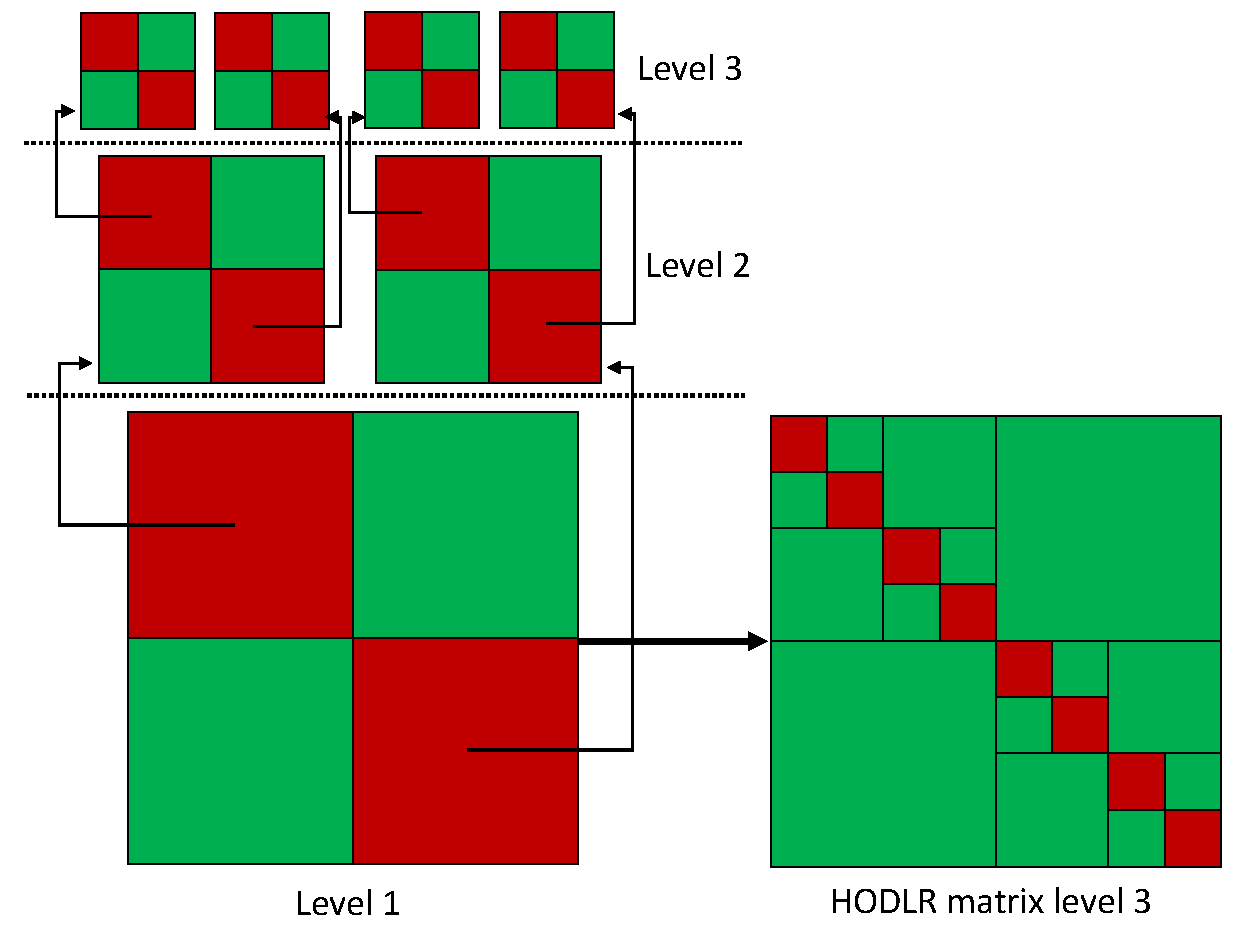
\includegraphics[width=0.38\textwidth]{./figures/hodlr_structure2.pdf}
\caption{Recursive construction of HODLR matrix of level 3. The red blocks are represented in dense format at all levels, while the green blocks are represented in low-rank format.}
\label{fig:hodlr-structure}
\end{figure}

\subsubsection{Tile Low-Rank Approximations}
Tile Low-Rank (TLR) approximation~\cite{akbudak2017tile,amestoy2015improving} is a flat approach that consists in splitting the dense matrix
into tiles of similar sizes. Fig.~\ref{fig:tlr-structure} shows an example of compressing 
an off-diagonal tile $T_{12}$ to two matrices $U_{12}$ and $V_{12}$,  
where the Singular Value Decomposition (SVD) is used to compress the dense matrix.
The most significant $k$ singular values are captured with their associated vectors, which
correspond to the rank of the tile.
Once each tile is compressed, the tile algorithm is expressed in terms of
tasks interconnected by their data dependencies. The original algorithm can then be translated into a
a Directed Acyclic Graph (DAG), where nodes are fine-grained computational tasks and edges express
their data dependencies. As implemented in the HiCMA library~\cite{hicma-soft}, the StarPU~\cite{augonnet2011starpu} dynamic runtime system
is used to orchestrate the scheduling of tasks with their data dependencies onto processing units.
The task-based programming model creates opportunities for look-ahead, which enables to maintain
high hardware occupancy.


% In the literature, parallel computation of dense linear algebra
% operations relies on two types of algorithms: block-based
% algorithms and tile-based algorithms. In block-based
% algorithms, the matrix is divided into a set of panels.
% Then, all the matrix operations are performed in two steps, panel factorization with level-2 BLAS operations, i.e., matrix-vector multiplication, is applied to a target panel, and trailing
% submatrix update where all panels transformation is
% applied to the rest of the matrix in the form of level-3 BLAS transformation, i.e., matrix-matrix multiplication.
% In tile-based algorithms, the matrix is divided into a set of
% tiles, and the matrix operations are defined as a set of
% sequential tasks that can be parallelized using a runtime system where the tasks dependencies are defined in the form of a Directed
% Acyclic Graph (DAG). This new form of computation provides more fine-grained computations that create opportunities for look-ahead to utilize the usage of existing hardware resources. Moreover, tile-based algorithms speed up parallel linear solvers  algorithms on
% manycore architectures and avoid the scalability problems with existing block-based algorithms.  LAPACK~\cite{anderson1999lapack} is an example
% of block-based software, and PLASMA~\cite{dongarra2019plasma}  and Chameleon are an example of tile-based software.

\begin{figure}[h]
\centering
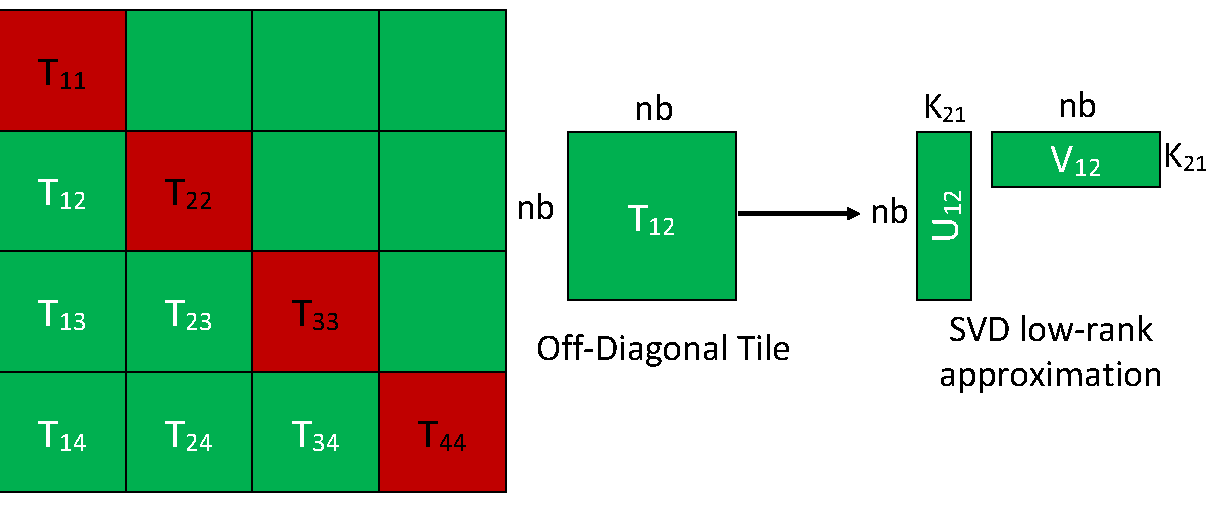
\includegraphics[width=0.38\textwidth]{./figures/tlr_graph.pdf}
\caption{An example of TLR approximation tile: diagonal tiles (in red) are dense. Off-diagonal tiles (in green) are represented as
low-rank approximation.}
\label{fig:tlr-structure}
\end{figure}

\section{Parallel TGH Non-Gaussian Modeling and Prediction}

This section explains our proposed parallel
implementation of the TGH non-Gaussian likelihoods
and predictions in exact, tile low-rank (TLR) approximation
and hierarchical off-diagonal low-rank (HODLR) approximation
format. We show the
distribution of the ranks in both TLR and HOLDR matrices
associated with TGH random fields compared to the dense matrix.



\subsection{Non-Gaussian Log-Likelihood Estimation}
Recalling the TGH random field log-likelihood function
in~(\ref{eq:Likelihood}), the log-likelihood estimation
operation involves generating a covariance 
matrix $\bm{R}_{\bm{\theta}_2}$ where $\bm{\theta}_2$ is the parameters of 
a given correlation function. Given a set of $n$ geospatial
locations, a selected covariance function can be used to
build an $n \times n$ covariance matrix. In this work, we
use the parametrizable Mat\'ern covariance function with
two parameters: $\phi$, the spatial range parameter, 
and $\nu$, the random field smoothness parameter.  
The other input parameter vector $\bm{\theta}_1= (\xi, \omega, g, h)^\top$ 
is used to transform the non-Gaussian measurement 
vector $\bm{Z}$  to a Gaussian vector $\bm{Z}_{\bm{\theta}_1}$. 

\begin{algorithm}[H]
\footnotesize
\caption{TGH Log-Likelihood Estimation.}
\label{algo:non-gaussian-model}
\begin{algorithmic}[1]
\STATE {\bf Input:} a set of locations $\bm{S} = \bm s_1,\ldots,\bm s_n$,   associated measurements $\bm{Z}_{\bm{\theta}_1,s_i}$, and current parameter vector $\bm{\theta}_1= (\xi, \omega, g, h)$.
\STATE {\bf Output:} the log-likelihood estimation for the current parameter vector $\bm{\theta}_1$
\STATE TGH transformation for $\bm{Z}_{\bm{\theta}_1,s_i} \leftarrow \tau_{g,h}^{-1} \bigg \{ \dfrac{t(\bm{s}_i) - \xi}{\omega} \bigg \}$ $\rightarrow$ eq(1)
\STATE  Generate covariance matrix $\bm{R}_{\bm{\theta}_2}$
$\rightarrow$ eq(5)
\STATE  POTRF($\bm{R}_{\bm{\theta}_2}$)  $\rightarrow$ Cholesky factorization
\STATE $determinant$ = Det($\bm{R}_{\bm{\theta}_2}$)
\STATE $S$ =  $\sum_{i=1}^n \log [ \exp(g z_{\bm{\theta}_1,\bm{s}_i})+g^{-1} \{ \exp(g z_{\bm{\theta}_1,\bm{s}_i}) -1 \} h z_{\bm{\theta}_1,\bm{s}_i}] -n \log \omega, $
\STATE TRSM ($\bm{R}_{\bm{\theta}_2}$, $\bm{Z}_{\bm{\theta}_1}$) $\rightarrow$ Triangular solve
\STATE  $dotproduct$ = (${\bm{Z}_{\bm{\theta}_1}}\times  \bm{Z}_{\bm{\theta}_1}$)
\STATE $llh$ = $-\frac{1}{2} (dotproduct + determinant)$ - $S$.


\end{algorithmic}
\end{algorithm}

Algorithm~\ref{algo:non-gaussian-model} presents the
TGH non-Gaussian log-likelihood estimation algorithm. 
The $\bm{Z}_{\bm{\theta}_1}$ vector transformation step
is performed first (line 1) with a given $\bm{\theta}_1$ parameter vector. Since the $\tau_{g,h}^{-1}(\cdot)$ has
no closed form, we use the Newton-Raphson method to
approximate the function for $Z_{\bm{\theta}_1}$ as follows:

\begin{equation}
\label{eq:newton}
\tau_{g,h}^{-1}(z_{\bm{\theta}_1, \bm{s}_i}) = \frac{t(\bm{s}_i) -\xi}{\omega}.
\end{equation}

%
% In line 2, the covariance  matrix $\bm{R}_{\bm{\theta}_2}$ is
% generated using the Mat\'ern covariance function in~(\ref{eq:matern}).
% In lines 3 and 4,  a matrix inverse and determinant are calculated by
% applying a Cholesky factorization operation. In line 5, the scalar
% quantity in~(\ref{eq:Likelihood}) is computed and stored in a scalar $S$.
% In line 6, a matrix-vector triangular solve operation is performed
% where the result is stored in $\bm{Z}_{\bm{\theta}_1}$. In line 7, a dot
% product operation is performed, producing a scalar $dotproduct$.
% In line 8, the log-likelihood function is calculated based on
% the  $dotproduct$, $determinant$, and $S$ scalar values.


The most time-consuming step in Algorithm~\ref{algo:non-gaussian-model} is the Cholesky 
factorization of the covariance matrix $\bm{R}_{\bm{\theta}_2}$ in line 3. 
 Therefore, we rely on the state-of-the-art
dense task-based library, i.e., Chameleon~\cite{chameleon-soft}, to perform the
linear algebra operations that appear in Algorithm~\ref{algo:non-gaussian-model}, including the Cholesky factorization of the
covariance matrix. Furthermore,  we exploit the data sparsity
structure of the covariance matrix and apply low-rank
approximation methods to reduce the overall 
complexity of the underlying linear algebra operations. 
In particular, we use TLR and HODLR matrix approximations to speed up the computation of the Cholesky factorization 
heavyweight operation while preserving the accuracy 
requirement of the application. 

\begin{figure}[t]
\centering
\begin{subfigure}{.15\textwidth}
  \centering
  \includegraphics[width=\linewidth]{{./figures/log_matern_0.7_0.5_0_2_0.2_0.2_8100_810_lr_5}.pdf}
   \caption{ $10^{-5}$.}
\end{subfigure}%
\begin{subfigure}{.15\textwidth}
  \centering
  \includegraphics[width=\linewidth]{{./figures/log_matern_0.7_0.5_0_2_0.2_0.2_8100_810_lr_7}.pdf}
  \caption{$10^{-7}$.}
\end{subfigure}%
\centering
\begin{subfigure}{.178\textwidth}
  \centering
  \includegraphics[width=\linewidth]{{./figures/log_matern_0.7_0.5_0_2_0.2_0.2_8100_810_lr_9}.pdf}
   \caption{ $10^{-9}$.}
\end{subfigure}
\caption{Rank distributions of a $8100 \times 8100$ non-Gaussian covariance TLR matrix using nb = 810 with TGH Mat\'ern parameters $\bm{\theta} = (0.96, 0.5, 0, 2, 0.5, 0.3)^\top$ under different accuracy levels.}
\label{fig:heatmap_tlr}
\end{figure}


\begin{figure}
     \centering
     \begin{subfigure}[b]{0.23\textwidth}
         \centering
         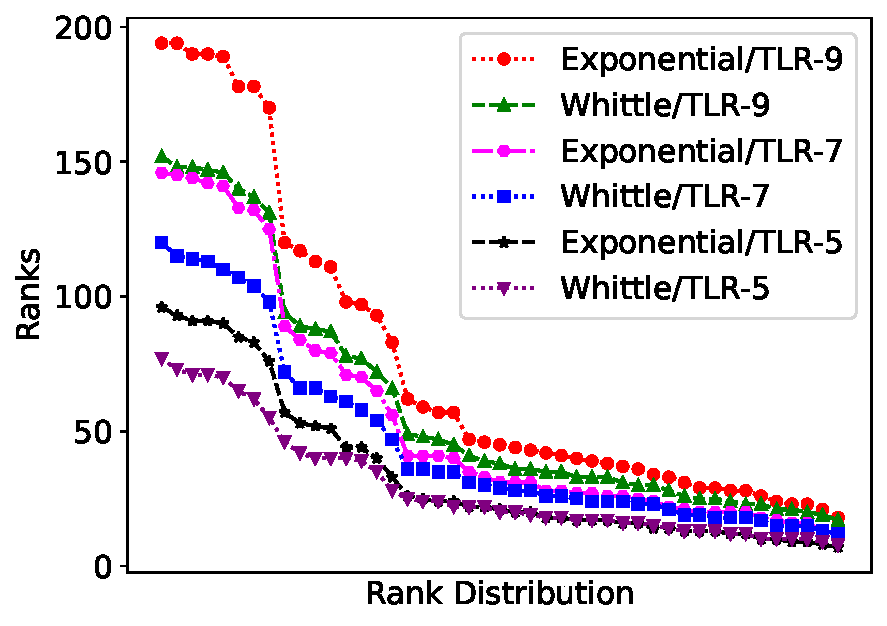
\includegraphics[width=\textwidth]{./figures/ranks-decay-8100.pdf}
         \caption{$N = 8100$ / $ts = 810$.}
         \label{fig:tlr-8100}
     \end{subfigure}
     \begin{subfigure}[b]{0.23\textwidth}
         \centering
         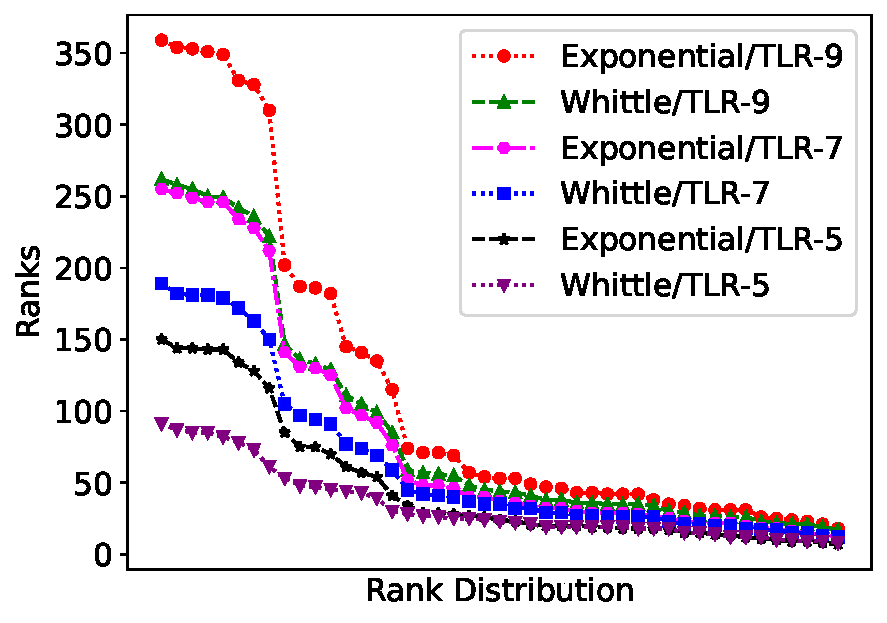
\includegraphics[width=\textwidth]{./figures/ranks-decay-32400.pdf}
         \caption{$N = 32400$ / $ts = 3240$.}
         \label{fig:tlr-32400}
     \end{subfigure}
        \caption{Decay of the ranks of different blocks with TLR approximation when using non-Gaussian Mat\'ern kernel with smoothness $\nu =0.5$ (Exponential kernel), and $\nu=1$ (Whittle kernel) and two matrix sizes.}
        \label{fig:tlr-deacy}
\end{figure}

\subsubsection{TLR Approximation of $\bm{R}_{\bm{\theta}_2}$}
The TLR approximation in HiCMA library compresses
the individual tile using
the SVD algorithm, where the ranks of the tiles represent
the most significant singular values and vectors in each off-diagonal tile~\cite{akbudak2017tile}. Therefore, the effectiveness of the TLR
mechanism depends on the ranks of the off-diagonal tiles
after compression, which in turn depends on the application's
accuracy requirements. Thus, we initially validate the potency 
of the TLR approximation with the TGH non-Gaussian modeling
by estimating the ranks corresponding to different accuracy levels, namely, TLR-5 ($10^{-5}$), TLR-7 ($10^{-7}$), and TLR-9 ($10^{-9}$). 
The required accuracy level of our application and the corresponding performance assessment is shown in detail in the performance
section. Herein, we just validate the effectiveness of using TLR
with our model.

Fig.~\ref{fig:heatmap_tlr} depicts the rank distribution
of a $8100 \times 8100$ covariance matrix generated by the
Mat\'ern covariance function shown in~(\ref{eq:matern}).  
As can be seen, the ranks of the off-diagonal tiles grow as the
tiles get closer to the diagonal with different TLR accuracy
levels with a monotonic increase of the ranks with tighter tolerance.
However, even with TLR-9, the ranks are still smaller than the
full dense tiles in the diagonal. The given example is drawn
from a synthetic set of TGH parameters $\bm{\theta} = (0.96, 0.5, 0, 2, 0.5, 0.3)^\top$, representing a medium correlation dependence between
the given spatial locations. We also examine other spatial
correlation strengths, and all of them show almost the same
ranks with different accuracy levels. We only observe a change
in the ranks with different smoothness values. 
For instance, in Fig.~\ref{fig:tlr-deacy}, we  report the 
decay of the ranks when using TLR approximation with 
different datasets with two data sizes, i.e., 8100 and 32400 using
different TLR accuracy levels and
a synthetic set of parameters $\bm{\theta} = (0.96, \nu, 0, 2, 0.5, 0.3)^\top$, 
where $\nu$ represents a rough field ($\nu=0.5$) and a smooth field ($\nu=1$). As shown, the ranks associated with rough fields have higher
ranks than smooth fields across all accuracy levels and the
two data sizes. The decaying figure also shows an increase in 
ranks when tile size is larger but preserving the same decaying
rate. Furthermore, we examined the ranks with different data
sizes and the same tile sizes, and we did not observe
any dramatic changes in ranks or ranks decaying. All the above observations show the advantage of using the TLR approximation
 in TGH modeling from the performance perspective.












\subsubsection{HODLR Approximation of $\bm{R}_{\bm{\theta}_2}$}
% The HODLR implementation in HODLRLIB compresses the
% matrix blocks using the rook pivoting algorithm and uses the
% KD-tree for hierarchical matrix partitioning. Each block is compressed individually, and the low-rank structure produces lower ranks
% compared to the dense format. As mentioned in TLR, the ranks
% values reflect the accuracy level of the compression and should be determined based on the application requirements.
Herein, we used also three accuracy levels, namely, HODLR-5 ($10^{-5}$), HODLR-7 ($10^{-7}$), and HODLR-9 ($10^{-9}$). 
Fig.~\ref{fig:heatmap_hodlr} depicts the rank distribution
of a $8100 \times 8100$ covariance matrix. Herein, we also use the medium correlation case to show the rank distribution. As shown by the figure, the matrix is divided into blocks in a hierarchical structure where the $leaf$  represents the size of matrices at leaf level. It is clearly shown that the smaller blocks have lower ranks, and at the higher structure levels of the matrix, the ranks increase. In red, the diagonal leaf blocks are kept dense. Furthermore, we do not observe any noticeable growth in ranks with larger $N$ when using the HODLR structure. Fig.~\ref{fig:hodlr-decay} shows the decay of the ranks in the case of HODLR matrices. The ranks drop faster than the TLR approximation because HODLR has smaller blocks at lower levels. We choose the size of leaf blocks:$100$ and $400$ 
with two matrix sizes. With larger leaf block size, the ranks
increases. As the LR approximation, increasing the matrix
size does not affect the ranks but compresses more blocks. 
The figure also shows the impact of the smoothness 
parameter $\nu$, which produces higher ranks in the rough field.

 
\begin{figure}[t]
\centering
\begin{subfigure}{.16\textwidth}
  \centering
  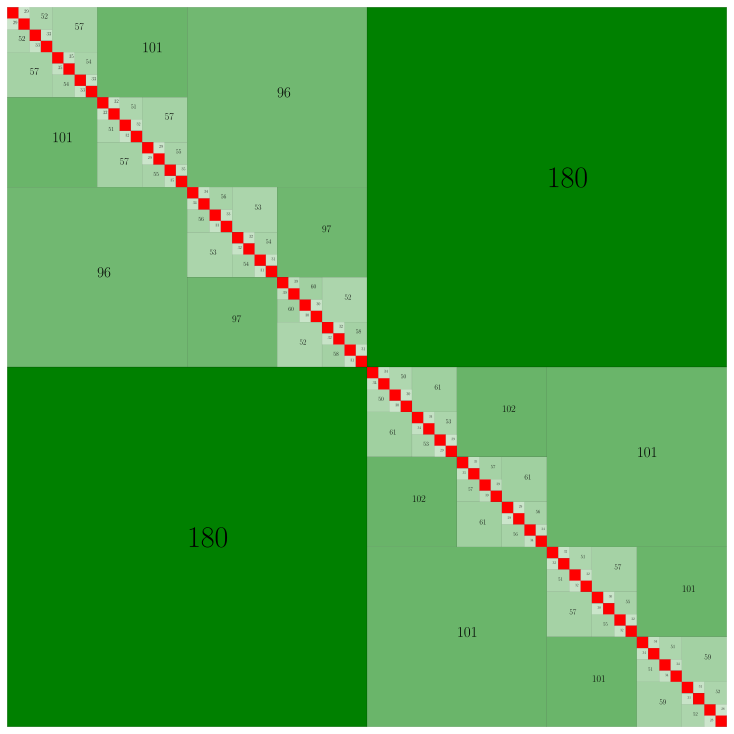
\includegraphics[width=\linewidth]{{./figures/image-8100-0.960000-0.500000-0.000000-2.000000-0.500000-0.300000-100--5.000000}.pdf}
   \caption{ $10^{-5}$.}
\end{subfigure}%
\begin{subfigure}{.16\textwidth}
  \centering
  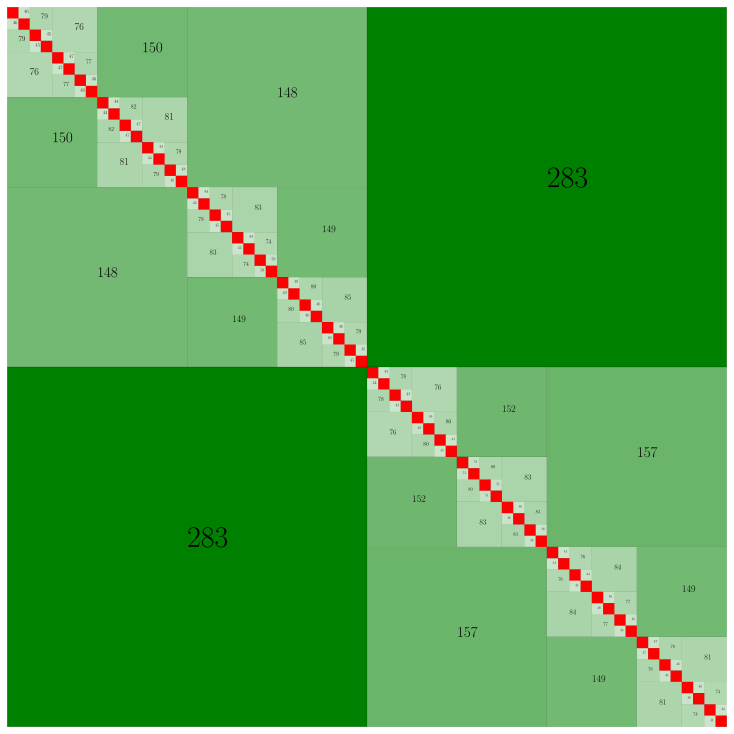
\includegraphics[width=\linewidth]{{./figures/image-8100-0.960000-0.500000-0.000000-2.000000-0.500000-0.300000-100--7.000000}.pdf}
   \caption{ $10^{-7}$.}
\end{subfigure}%
\centering
\begin{subfigure}{.16\textwidth}
  \centering
  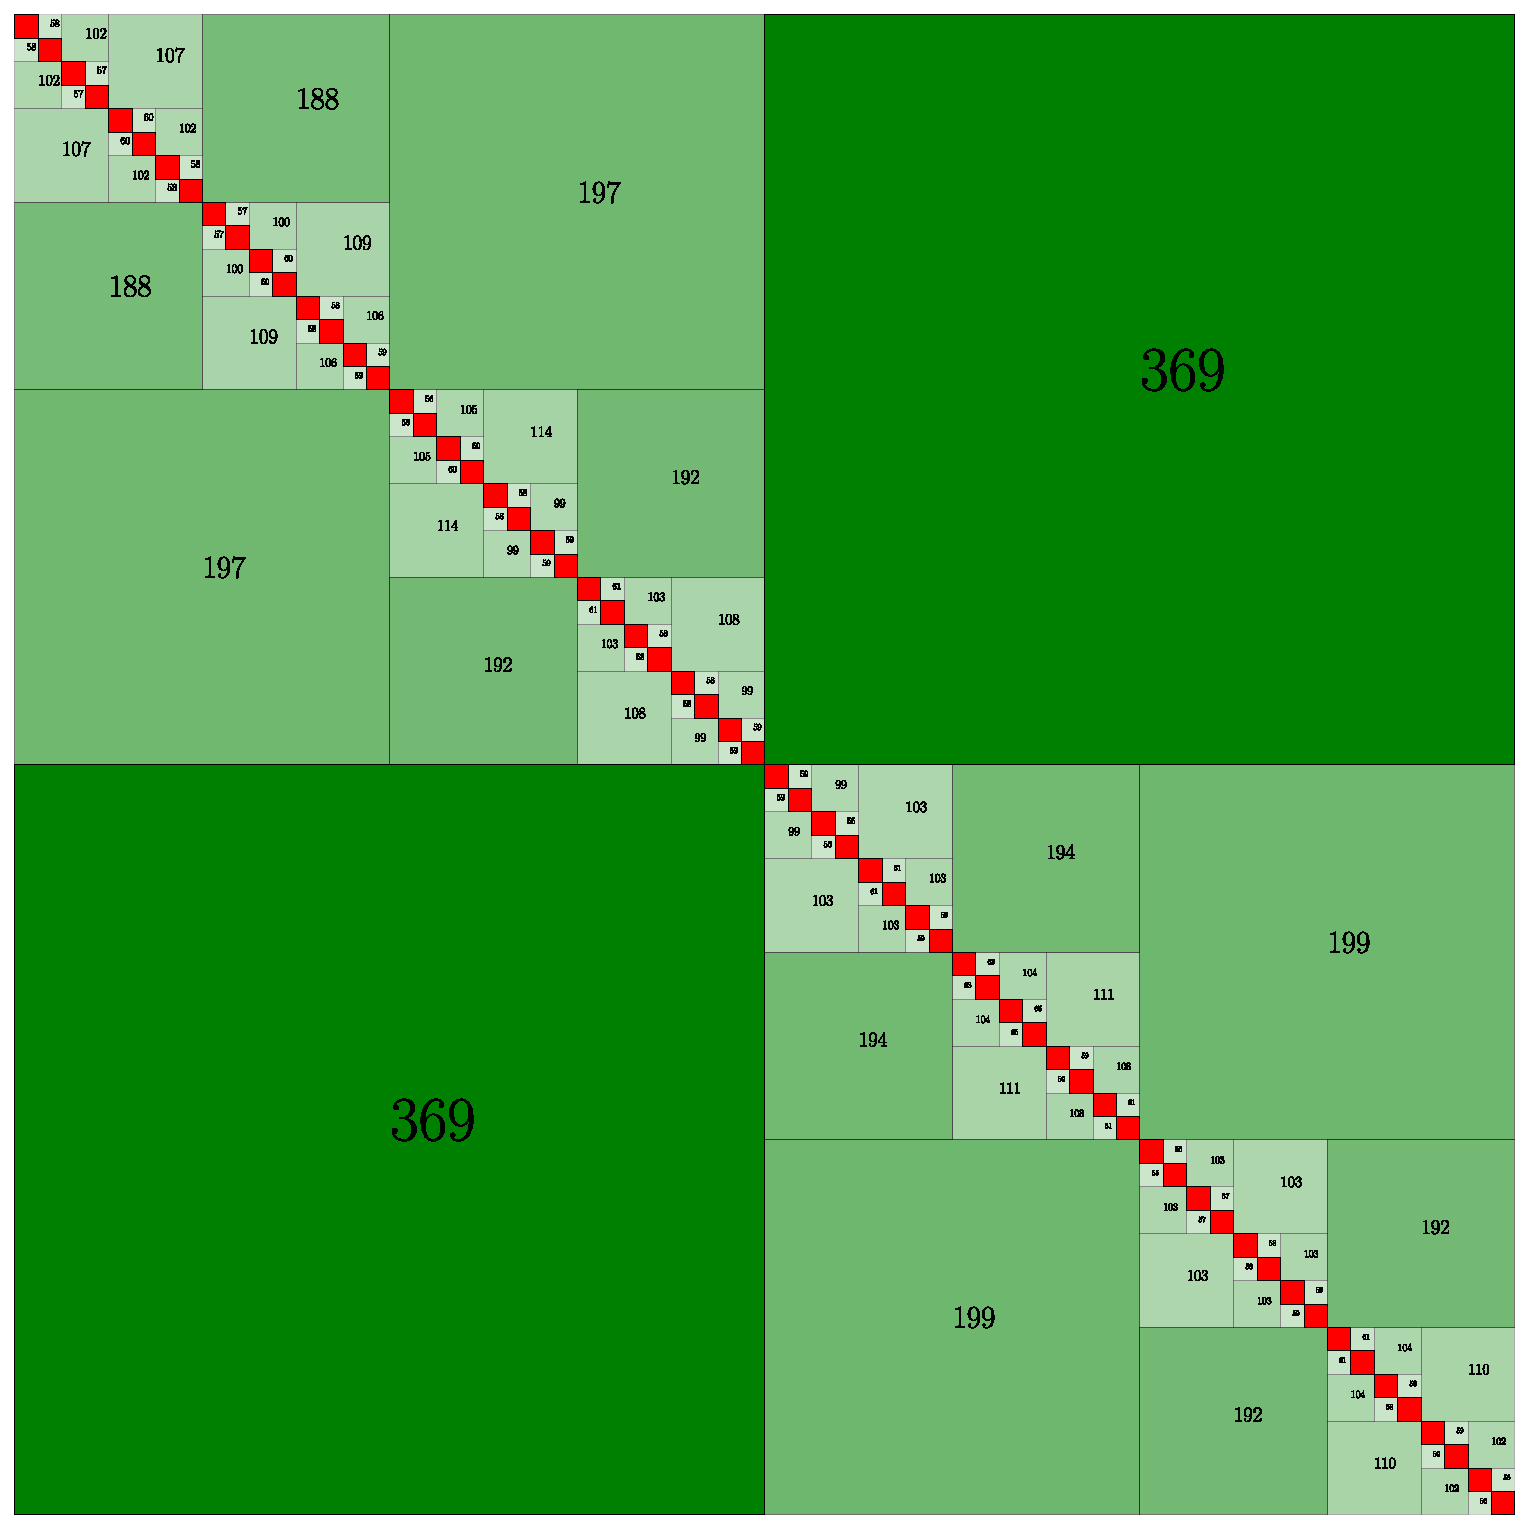
\includegraphics[width=\linewidth]{{./figures/image-8100-0.960000-0.500000-0.000000-2.000000-0.500000-0.300000-100--9.000000}.pdf}
   \caption{ $10^{-9}$.}
\end{subfigure}
\caption{Rank distributions of a $8100 \times 8100$ non-Gaussian covariance HODLR matrix using leaf = 100 with TGH Mat\'ern parameters $\bm{\theta} = (0.96, 0.5, 0, 2, 0.5, 0.3)^\top$ under different accuracy levels.}
\label{fig:heatmap_hodlr}
\end{figure}

\begin{figure}
     \centering
     \begin{subfigure}[b]{0.23\textwidth}
         \centering
         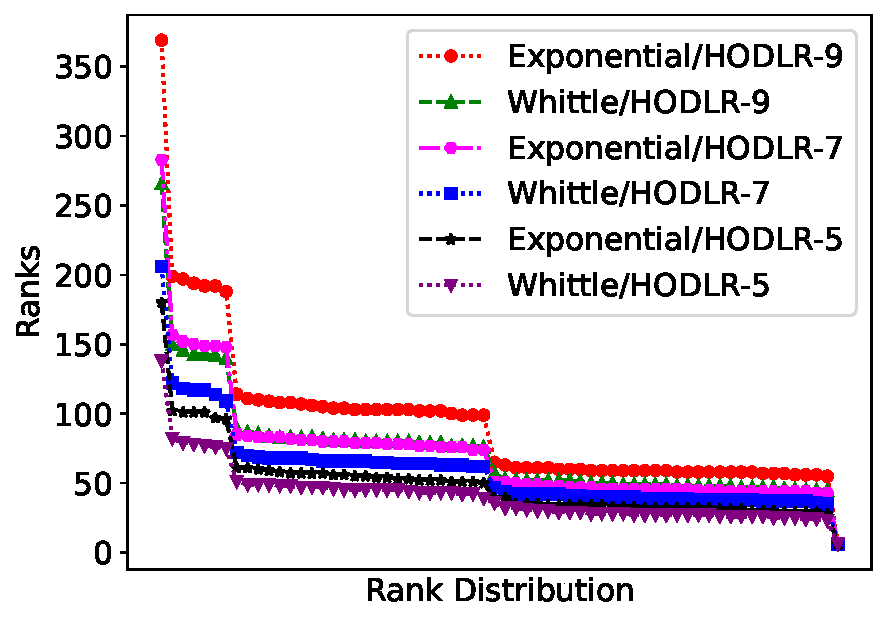
\includegraphics[width=\textwidth]{./figures/ranks-decay-8100-hodlr.pdf}
         \caption{$N = 8100$ / $leaf = 100$.}
         \label{fig:hodlr-decay-8100}
     \end{subfigure}
     \begin{subfigure}[b]{0.23\textwidth}
         \centering
         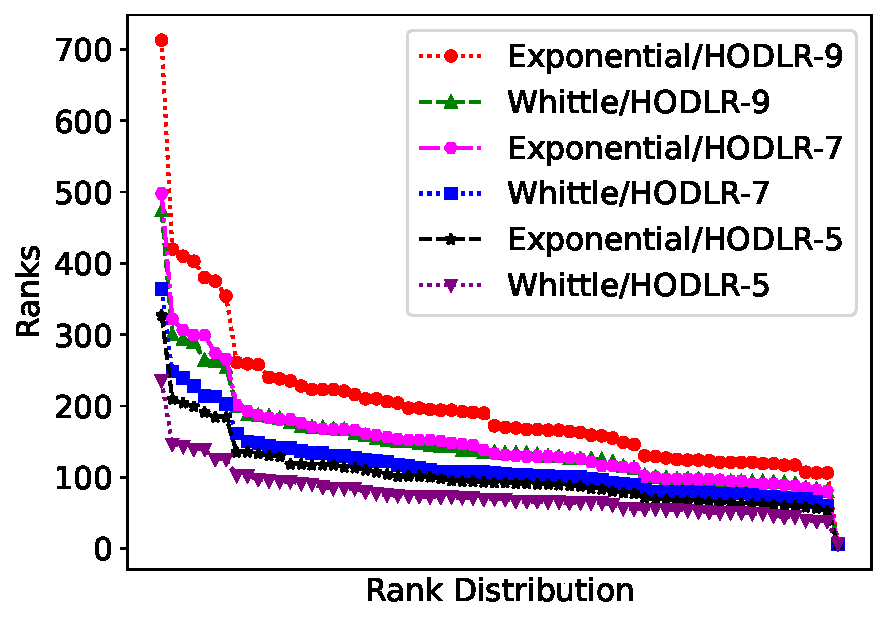
\includegraphics[width=\textwidth]{./figures/ranks-decay-32400-hodlr.pdf}
         \caption{$N = 32400$ / $leaf = 400$.}
         \label{fig:hodlr-decay-32400}
     \end{subfigure}
        \caption{Decay of the ranks of different blocks with HODLR approximation when using non-Gaussian Mat\'ern kernel with smoothness $\nu =0.5$ (Exponential kernel), and $\nu=1$ (Whittle kernel) and two matrix sizes.}
        \label{fig:hodlr-decay}
\end{figure}


\subsection{TGH Non-Gaussian Prediction}
The optimization process of the likelihood function aims
at tuning the TGH parameter vectors, i.e., $\widehat{\bm{\theta}}_1$
 and $\widehat{\bm{\theta}}_2$. These parameters are used to
 predict missing measurements at a set of locations using 
 Equation~(\ref{eq:prediction}). Algorithm~\ref{algo:non-gaussian-pred} 
shows in detail the numerical steps to predict missing
 values using the two tuned parameter vectors. 
%  Line 1 includes
%  the non-Gaussian to Gaussian transformation of the $\bm{Z}_{obs}$
%  vector using the Newton-Raphson method. In line 2, the  $\bm{R}_{\widehat{\bm{\theta}}_2}$ covariance matrix of the observed
%  locations is generated. In line 3, another covariance matrix of
%  both the observed and the missing locations $\bm{r}_{\theta_2}$ is generated. In lines 6 and 7, two triangular solve  operations are
%  performed to compute the expression $\bm{r}_{\widehat{\bm{\theta}}_2}^\top \bm{R}_{\widehat{\bm{\theta}}_2}^{-1} \bm{r}_{\widehat{\bm{\theta}}_2}$. Line 8 shows a matrix-vector multiplication operation while line 9
% shows a matrix-matrix multiplication to compute the $tmp_1$
% vector and the $tmp_2$ matrix.
Line 4 accounts for most of the algorithmic complexity as it involves the Cholesky-based
solver of the covariance matrix. This algorithm performs prediction of the missing data
on the location $\bm{s}_k$.

\begin{algorithm}[H]
\footnotesize
\caption{TGH Prediction.}
\label{algo:non-gaussian-pred}
\begin{algorithmic}[1]
\STATE {\bf Input:} a set of locations $\bm{S} = \bm s_1,\ldots,\bm s_n$,   associated measurements $\bm{Z}_{\bm{\theta}_1,s_i}$, and estimated parameter vector $\widehat{\bm{\theta}_2}$.
\STATE {\bf Output:} the predicted values at missing locations $\widehat{Y}^{opt}$.
\STATE TGH transformation for $\bm{Z}_{obs,s_i} \leftarrow \tau_{g,h}^{-1} \bigg \{ \dfrac{t(\bm{s}_i) - \xi}{\omega} \bigg \}$
\STATE  Generate covariance matrix $\bm{R}_{\widehat{\bm{\theta}}_2}$ $\rightarrow$ eq(5)
    \STATE Generate covariance matrix $\bm{r}_{\widehat{\bm{\theta}}_2}$  $\rightarrow$ eq(5)
\STATE  POSV ($\bm{R}_{\widehat{\bm{\theta}}_2}, \bm{Z}_{obs})$ $\rightarrow$ System of linear equations solver.
	%\FOR{k = 1 to $n_{miss}$} 
    % POTRF
        \STATE CPY ($\bm{r}_{\widehat{\bm{\theta}}_2}$, $\bm{rcpy}_{\widehat{\bm{\theta}}_2}$) 
    \STATE TRSM ($\bm{R}_{\widehat{\bm{\theta}}_2}, \bm{r}_{\widehat{\bm{\theta}}_2}$) $\rightarrow$ Triangular solve
        \STATE TRSM ($\bm{R}_{\widehat{\bm{\theta}}_2}^\top, \bm{r}_{\widehat{\bm{\theta}}_2}$) $\rightarrow$ Triangular solve
                \STATE $\bm{tmp_1}$ = GEMV$(\bm{rcpy}_{\widehat{\bm{\theta}}_2}, \bm{Z}_{obs})$ $\rightarrow$ Matrix-vector multiplication 
                \STATE $\bm{tmp_2}$ = GEMM$ (\bm{rcpy}_{\widehat{\bm{\theta}}_2}, \bm{r}_{\widehat{\bm{\theta}}_2})$ $\rightarrow$ Matrix-matrix multiplication 
        \FOR{$k = 1$ to $n_{miss}$}
                \STATE $\tilde{\mu}$ =  $\bm{tmp_1}[k]$
        \STATE $\tilde{\sigma_2}$ = $1-\bm{tmp_2}[k]$
               %\STATE $\widehat{Y_1}^{opt}(\bm{s}_k)=\xi + \bm{X}(\bm{s}_k)^T  \bm{\beta} + \omega t_{g,h}(\tilde{\mu})$
        \STATE $\widehat{Y}^{opt}(\bm{s}_k)=\xi +  \frac{\omega}{g\sqrt{1-h\tilde{\sigma}^2}} \exp{\frac{h\tilde{\mu}^2}{2(1-h\tilde{\sigma}^2)}}      \times [\exp{\frac{g^2\tilde{\sigma}_2+2g\tilde{\mu}}{2(1-h\tilde{\sigma}^2)}-1}] $
  \ENDFOR
\end{algorithmic}
\end{algorithm}


Using low-rank approximation in the form of TLR or HODLR for both $\bm{R}_{\widehat{\bm{\theta}}_2}$ and $\bm{r}_{\widehat{\bm{\theta}}_2}$  in
 Algorithm~\ref{algo:non-gaussian-pred} can help
in reducing the complexity of the TGH prediction algorithm
similar to the likelihood estimation operation. In the following
section, we give a detailed performance assessment of different
proposed TGH implementations.

\section{Performance Results}
This section assesses the accuracy and performance of 
different proposed TGH non-Gaussian implementations
using synthetic and real precipitation datasets with different sizes and
characteristics. 

% We conduct a set of experiments with different objectives: 1) assess the estimation of the non-Gaussian
% parameters using exact, TLR, and HODLR approaches; 2) evaluate
% the prediction accuracy of the TGH random fields compared
% to the Gaussian random fields on synthetic datasets; and 3) assess
% the quality of the TGH modeling and prediction on a real
% precipitation dataset in the context of climate and
% environmental applications.




\subsection{Testbed and Methodology}
The assessment of the exact and approximate implementations of TGH non-Gaussian modeling and prediction has been conducted  on
Intel and AMD chips to highlight our software
portability: a 28-core dual-socket Intel Xeon IceLake
Gold 6330 CPU running at 2.00 GHz, and a 64-core dual-socket AMD EPYC Milan 7713 CPU running at 2.00 GHz. For the distributed-memory experiments, we use a Cray XC40
system with 6,174 dual-socket compute nodes based on 16-
core Intel Haswell processors running at 2.3 GHz. Each node
has 128 GB of DDR4 memory. The system has a total of
197,568 processor cores and 790 TB of aggregate memory.

Our implementation enables performance portability as long as an optimized BLAS/LAPACK library is available on the target system. On our testbed systems, we rely on Intel MKL v2020.0.166 as the optimized BLAS/LAPACK library to link against the necessary optimized numerical routines for our implementations. We compile our exact and TLR code using Chameleon and HiCMA linear algebra libraries with  GCC V11.1, HWLOC v2.5.0, StarPU v1.3.8,  GSL v2.7,
and NLopt v2.6.2 optimization libraries. For HODLR-based implementation, we use HODLRLIB, compiled it with GCC V11.1, and linked it with GSL v2.7 and NLopt v2.6.2. All computations are carried out in double-precision arithmetic.%, and each run has been repeated three times.

The accuracy and qualitative analyses are performed using synthetic and real datasets, i.e., the precipitation dataset of Germany. We use the daily average precipitation of Germany in January of the year 2021. The data is collected by Kaspar et al. \cite{kaspar2013monitoring} and covers the whole of Germany with a spatial resolution of $1$ km $\times$ $1$ km. The daily average precipitation is given in mm. Because of this high spatial resolution, the total number of locations is $n = 358303$. To make the data stationary, we remove the mean of the daily average precipitation of January over the year 2000 to 2020 from the data. So, the data can be interpreted as the excess daily average precipitation for January of 2021. The spatial image of the data is given in Fig.~\ref{fig:data_image}.
\begin{figure}[h]
\centering
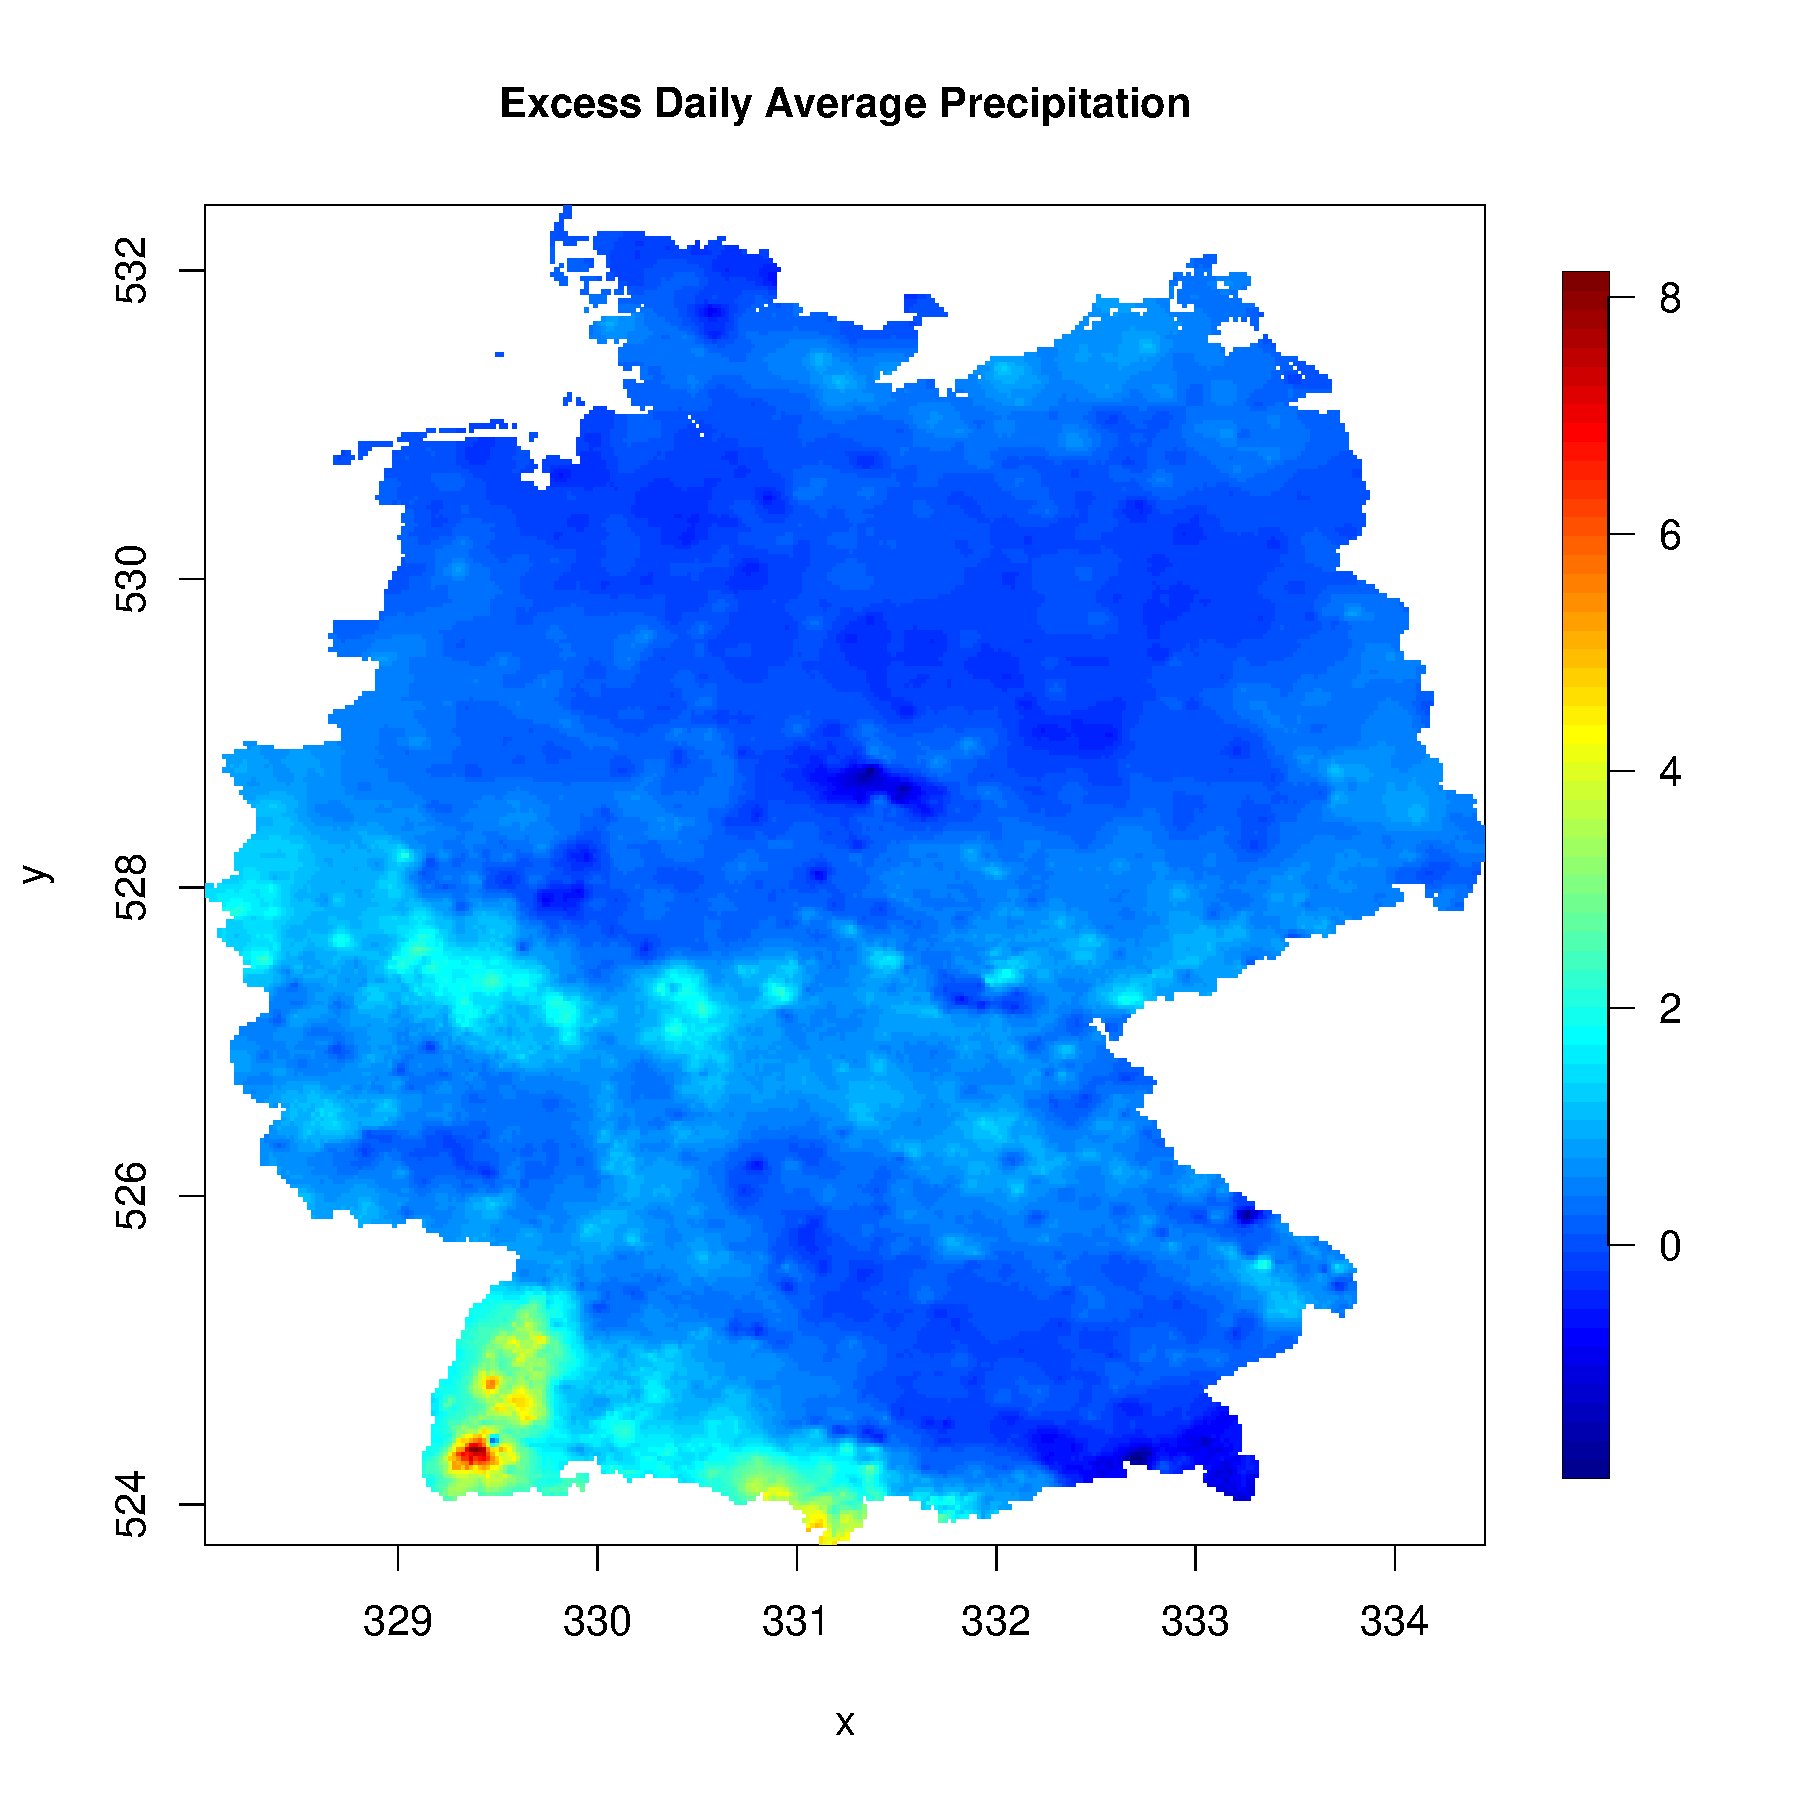
\includegraphics[width=0.7\linewidth]{./figures/data_spatial_image.pdf}
  \caption{Spatial image of the excess daily average precipitation (in mm) of January, 2021 on 358303 locations over Germany.
}
  \label{fig:data_image}
\end{figure}

\subsection{TLR/HODLR Accuracy Estimation Assessment}
%%%%%%%%%%%%%%%%
In this section, we demonstrate the accuracy of the MLE obtained using synthetic datasets. We generate $20164$ random observations from a TGH random field defined in \eqref{eq:TGH_random_field} on the  $[0,1]\times[0,1]$ square in the following four setups, with latent correlation function as in \eqref{eq:matern}:
\begin{enumerate}
\item[(a)] $\xi = 0$, $\omega = 2$, $g = 0.2$, $h = 0.2$, $\nu = 0.5$, and $\phi = 0.42$, with effective range $0.3$;
\item[(b)] $\xi = 0$, $\omega = 2$, $g = 0.2$, $h = 0.2$, $\nu = 0.5$, and $\phi = 0.7$, with effective range $0.5$;
\item[(c)] $\xi = 0$, $\omega = 2$, $g = 0.5$, $h = 0.3$, $\nu = 0.5$, and $\phi = 0.96$, with effective range $0.5$;
\item[(d)] $\xi = 0$, $\omega = 2$, $g = 0.2$, $h = 0.2$, $\nu = 0.5$, and $\phi = 0.98$, with effective range $0.7$.
\end{enumerate}


The effective range is the distance at which the correlation between two points becomes less than $0.05$. Given the other parameters, we find $\phi$ for different setups by changing the effective range. We use the correlation function of the TGH random field, given in \cite{xu2017tukey}, for evaluating $\phi$ in different setups. 
For each of these four setups, we estimate the parameters by maximizing the likelihood function given in \eqref{eq:Likelihood}. We compute the log-likelihood with TLR and HODLR with different accuracies. We repeat the procedure 100 times for both TLR and HODLR and their different accuracies. Moreover, we do the same with the exact log-likelihood. We present the boxplots of the estimated parameter values for different setups and different computation techniques in Fig.~\ref{fig:boxplot}. We used three accuracy levels for both HODLR (i.e., HODLR-5, HODLR-7, and HODLR-9) and TLR (i.e., TLR-5, TLR-7, and TLR-9) compared to the exact estimation (i.e., Exact).


The boxplots suggest that the estimation accuracy does not vary much with the different parameter setups. It is also worth noting that the estimation accuracy increases if we increase the accuracy of TLR or HODLR. Our result also shows that TLR works better for TGH non-Gaussian model estimation compared to HODLR over different accuracies. As expected for higher accuracy, the difference between TLR, HODLR, and exact becomes negligible.


%%%%%%%%%%%

%\begin{figure*}[htp!]
%\centering
%\begin{subfigure}{.5\textwidth}
% % \centering
%  \includegraphics[width=\linewidth]{{./figures/boxplot_0.420000_0.200000_0.200000}.pdf}
%  \vspace{-8mm}
%   \caption{ $\xi = 0$, $\omega = 2$, $g = 0.2$, $h = 0.2$, $\nu = 0.5$, and $\phi = 0.42$.}
%\end{subfigure}
%\begin{subfigure}{.5\textwidth}
%  %\centering
%  \includegraphics[width=\linewidth]{{./figures/boxplot_0.700000_0.200000_0.200000}.pdf}
%\vspace{-8mm}  
%  \caption{  $\xi = 0$, $\omega = 2$, $g = 0.2$, $h = 0.2$, $\nu = 0.5$, and $\phi = 0.7$.}
%\end{subfigure}%
%
%%\centering
%\begin{subfigure}{.5\textwidth}%
%  %\centering
%  \includegraphics[width=\linewidth]{{./figures/boxplot_0.960000_0.500000_0.300000}.pdf}
%  \vspace{-8mm}
%   \caption{$\xi = 0$, $\omega = 2$, $g = 0.5$, $h = 0.3$, $\nu = 0.5$, and $\phi = 0.96$.}
%\end{subfigure}
%\begin{subfigure}{.5\textwidth}
%  %\centering
%  \includegraphics[width=\linewidth]{{./figures/boxplot_0.980000_0.200000_0.200000}.pdf}
%  \vspace{-8mm}
%  \caption{  $\xi = 0$, $\omega = 2$, $g = 0.2$, $h = 0.2$, $\nu = 0.5$, and $\phi = 0.98$.}
%\end{subfigure}
%\caption{Boxplots of parameter estimates under the HODLR, TLR, and exact log-likelihood computation. The true parameters are indicated by the red lines.}
%\label{fig:boxplot}
%\end{figure*}

\begin{figure*}[htp!]
\centering
%\begin{subfigure}{0.5\textwidth}
%  \centering
%  \includegraphics[width=\linewidth]{./figures/boxplot_0.420000_0.200000_0.200000.pdf}
%   \vspace{-8mm}
%   \caption{ $\xi = 0$, $\omega = 2$, $g = 0.2$, $h = 0.2$, $\nu = 0.5$, and $\phi = 0.42$.}
%\end{subfigure}
\begin{subfigure}{0.45\textwidth}%
  \centering
  \includegraphics[width=\linewidth]{./figures/boxplot_0.420000_0.200000_0.200000.pdf}
 % \vspace{-8mm}  
  \caption{ $\xi = 0$, $\omega = 2$, $g = 0.2$, $h = 0.2$, $\nu = 0.5$, and $\phi = 0.42$.}
\end{subfigure}%
\hspace{4mm}
\begin{subfigure}{0.45\textwidth}%
  \centering
  \includegraphics[width=\linewidth]{./figures/boxplot_0.700000_0.200000_0.200000.pdf}
% \vspace{-8mm}
   \caption{  $\xi = 0$, $\omega = 2$, $g = 0.2$, $h = 0.2$, $\nu = 0.5$, and $\phi = 0.7$.}
\end{subfigure}

\centering
\begin{subfigure}{0.45\textwidth}%
  \centering
  \includegraphics[width=\linewidth]{./figures/boxplot_0.960000_0.500000_0.300000.pdf}
 %  \vspace{-8mm}
  \caption{$\xi = 0$, $\omega = 2$, $g = 0.5$, $h = 0.3$, $\nu = 0.5$, and $\phi = 0.96$.}
\end{subfigure}%
\hspace{4mm}
\begin{subfigure}{0.45\textwidth}%
  \centering
  \includegraphics[width=\linewidth]{./figures/boxplot_0.980000_0.200000_0.200000.pdf}
 %  \vspace{-8mm}
  \caption{  $\xi = 0$, $\omega = 2$, $g = 0.2$, $h = 0.2$, $\nu = 0.5$, and $\phi = 0.98$.}
\end{subfigure}%
\caption{Boxplots of parameter estimates under the HODLR (H), TLR (T), and exact (E) log-likelihood computation. The true parameters are indicated by the red lines.}
\label{fig:boxplot}
\end{figure*}

\subsection{Evaluation of Prediction with TGH Random Fields}
\label{sec:pit}
We check the validity of our PIT assessment tool of the TGH non-Gaussian model. In this simulation study, we generate observations with parameter of setup (a) from the previous section and fit both Gaussian and TGH non-Gaussian models. We create the PIT histogram using the method discussed in Section~\ref{sec:pit}. Fig.~\ref{fig:PIT_synthetic} suggests that the PIT histogram obtained by fitting the Gaussian model is not at all a representation of a uniform distribution. To create a single measure of model adequacy, we introduce the mean divergence distance (MDD) from the PIT histograms. The MDD is defined as the average squared divergence of the length of the bars of the histogram from the value $1$ (uniform density): the smaller the MDD, the better the fitted model. The MDD of both models is reported in Fig.~\ref{fig:PIT_synthetic}. As expected, the TGH non-Gaussian model performs better than the Gaussian model for this synthetic data.
\begin{figure}[h]
\centering
\begin{subfigure}{.25\textwidth}
  \centering
  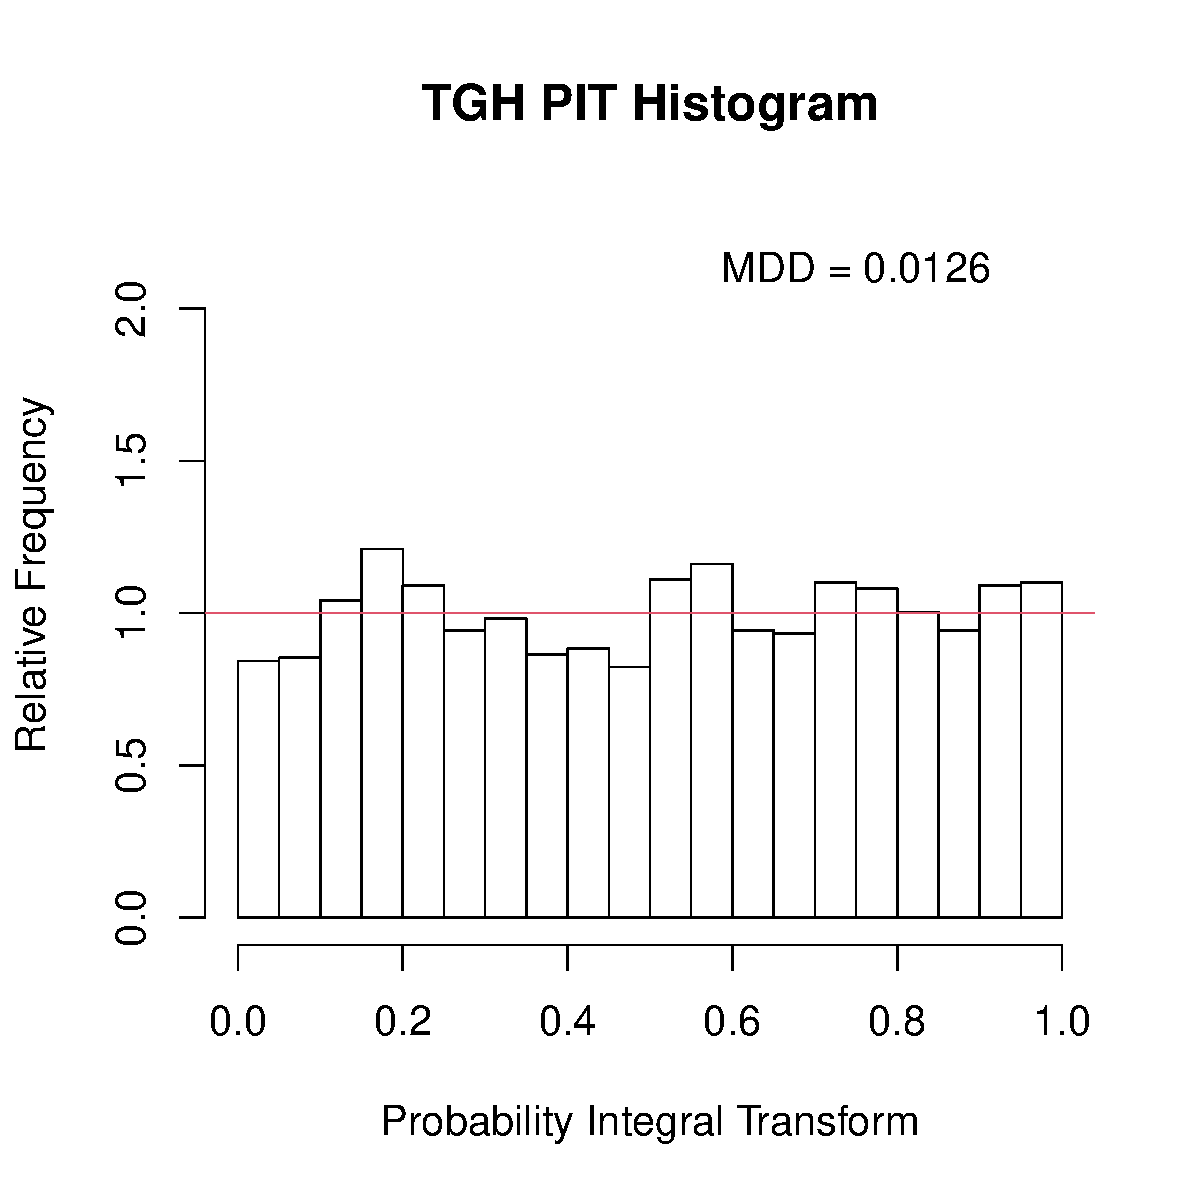
\includegraphics[width=\linewidth]{./figures/PIT_TGH.pdf}
   \caption{TGH non-Gaussian.}
\end{subfigure}%
\begin{subfigure}{.25\textwidth}
  \centering
  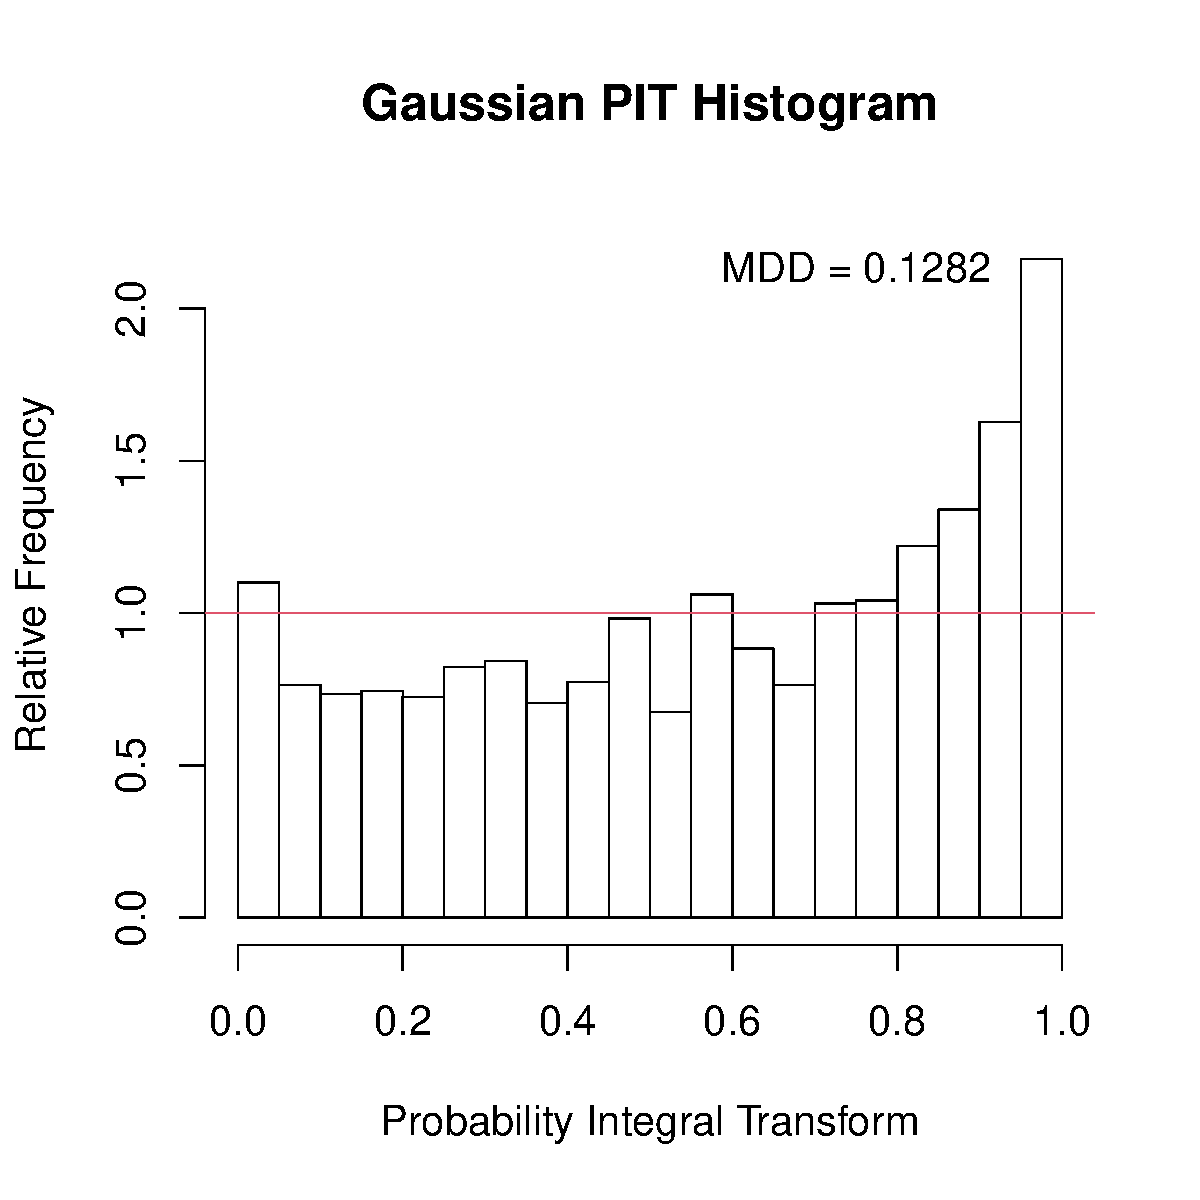
\includegraphics[width=\linewidth]{./figures/PIT_Gau.pdf}
  \caption{Gaussian.}
\end{subfigure}
  \caption{PIT histograms for predictive distribution with the same TGH synthetic dataset.}
  \label{fig:PIT_synthetic}
\end{figure}




\subsection{Precipitation Data Assessment}  
We fit both Gaussian and TGH non-Gaussian models to a subsample of 
size $300K$ locations. The estimated parameter values are 
given in Table~\ref{table:estimates}. The estimates of the 
parameters $g$ and $h$ from the TGH model indicate that 
the data is far from a Gaussian random field. This claim has 
been justified by our PIT assessment tool. Based on these 
estimates, we predict the values for $30K$ locations, separate 
from the training subsample. We produce the PIT histogram for 
both the fitted model based on the testing data. The PIT histograms
are given in Fig.~\ref{fig:PIT_real}. We can see from Fig.~\ref{fig:PIT_real} that the PIT histogram obtained from the Gaussian model does not correspond to a uniform distribution. The PIT
from the TGH non-Gaussian model shows a uniform distribution where
the Gaussian model MDD is $0.5434$ while TGH model MDD is $0.0290$. This observation leads us to the conclusion that the fitted TGH non-Gaussian model 
is appropriate to explain the variability of the data, as seen in the precipitation dataset
on the bottom-left location in Fig.~\ref{fig:data_image}. 

%We also report the MSPE and MDD for both models in Table \ref{table:MSPE}. Although the MSPE are essentially identical (very slightly better for the Gaussian model), this does not mean that the Gaussian model is more appropriate thanthe TGH model for this case. Here MDD should be used for a single measure of model adequacy.
\begin{table}
\begin{center}
\begin{tabular}{ |c|c|c|c|c|c|c| } 
 \hline
 Model & $\phi$ & $\nu$ & $\xi$ & $\omega$& $g$ & $h$  \\
 \hline 
Gaussian & $10.36$ & $0.57$ & $0.26$ & $1.04$ & -  & -   \\
 \hline
 TGH & $10.78$ & $0.64$ & $-0.37$ & $0.85$ & $-1.69$ & $0.65$ \\
 \hline
 \end{tabular}
\end{center}
\caption{Parameter estimates for Gaussian and TGH non-Gaussian models with the real dataset.}
\label{table:estimates}
\end{table}

%\begin{table}
%\begin{center}
%\begin{tabular}{ |c|c|c|c| } 
%\hline
% Model   & MSPE & MDD \\
%\hline 
%Gaussian & $0.00144$ & $0.5434$ \\
% \hline
% TGH  & $0.00146$ & $0.0290$ \\
%  \hline
%\end{tabular}
%\end{center}
%\caption{MSPE and MDD for Gaussian and TGH model}
%\label{table:MSPE}
%\end{table}

\begin{figure}[h]
\centering
\begin{subfigure}{.25\textwidth}
  \centering
  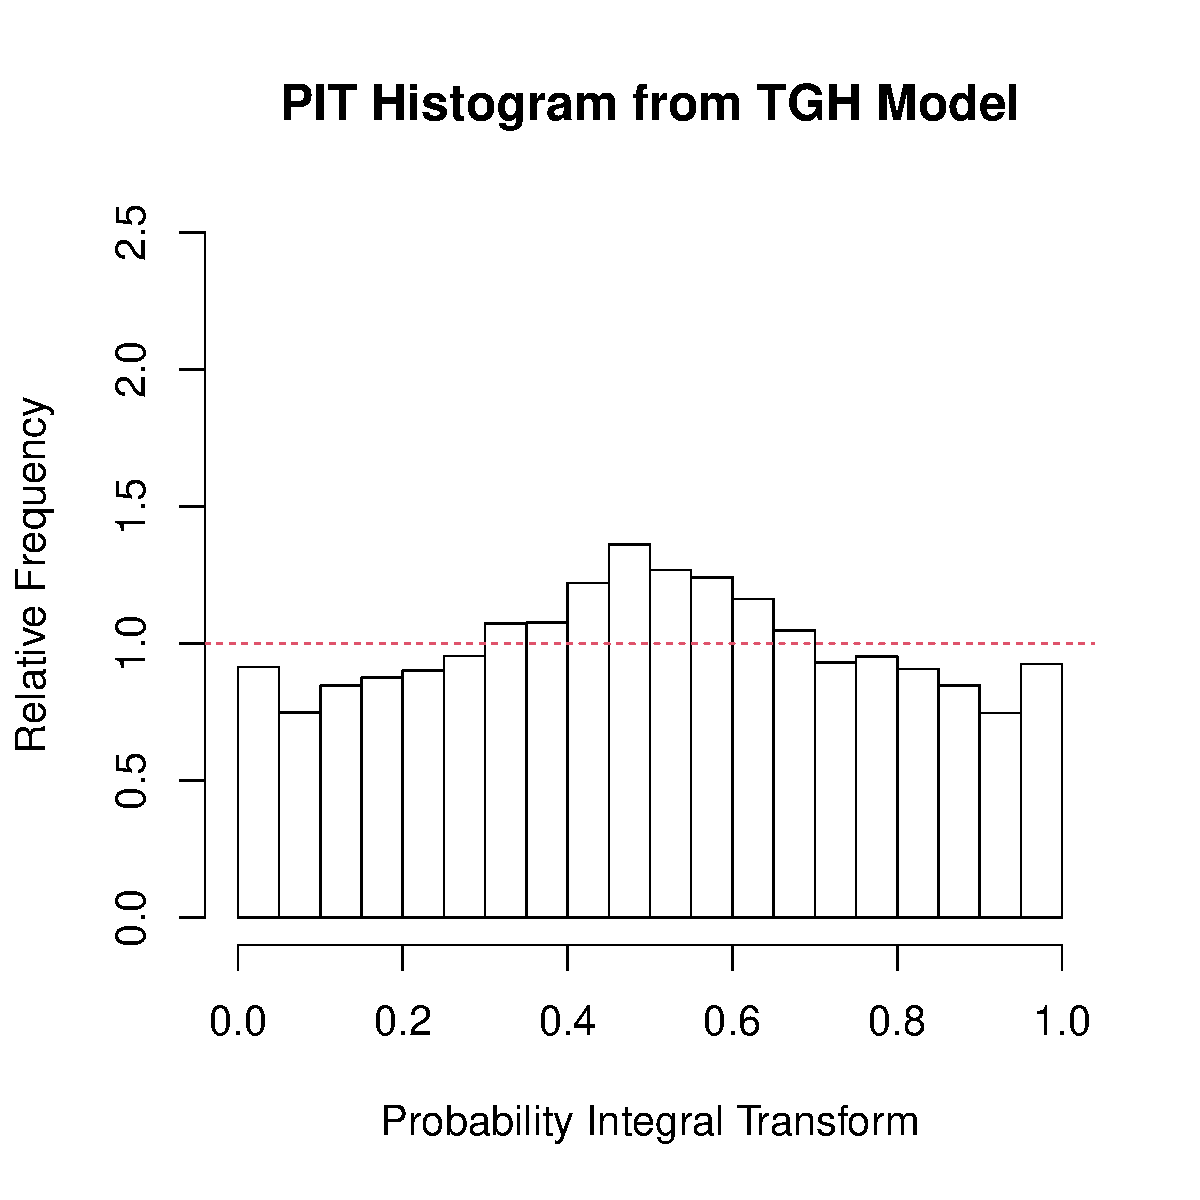
\includegraphics[width=\linewidth]{./figures/PIT_real_nongaussian.pdf}
   \caption{TGH non-Gaussian model.}
\end{subfigure}%
\begin{subfigure}{.25\textwidth}
  \centering
  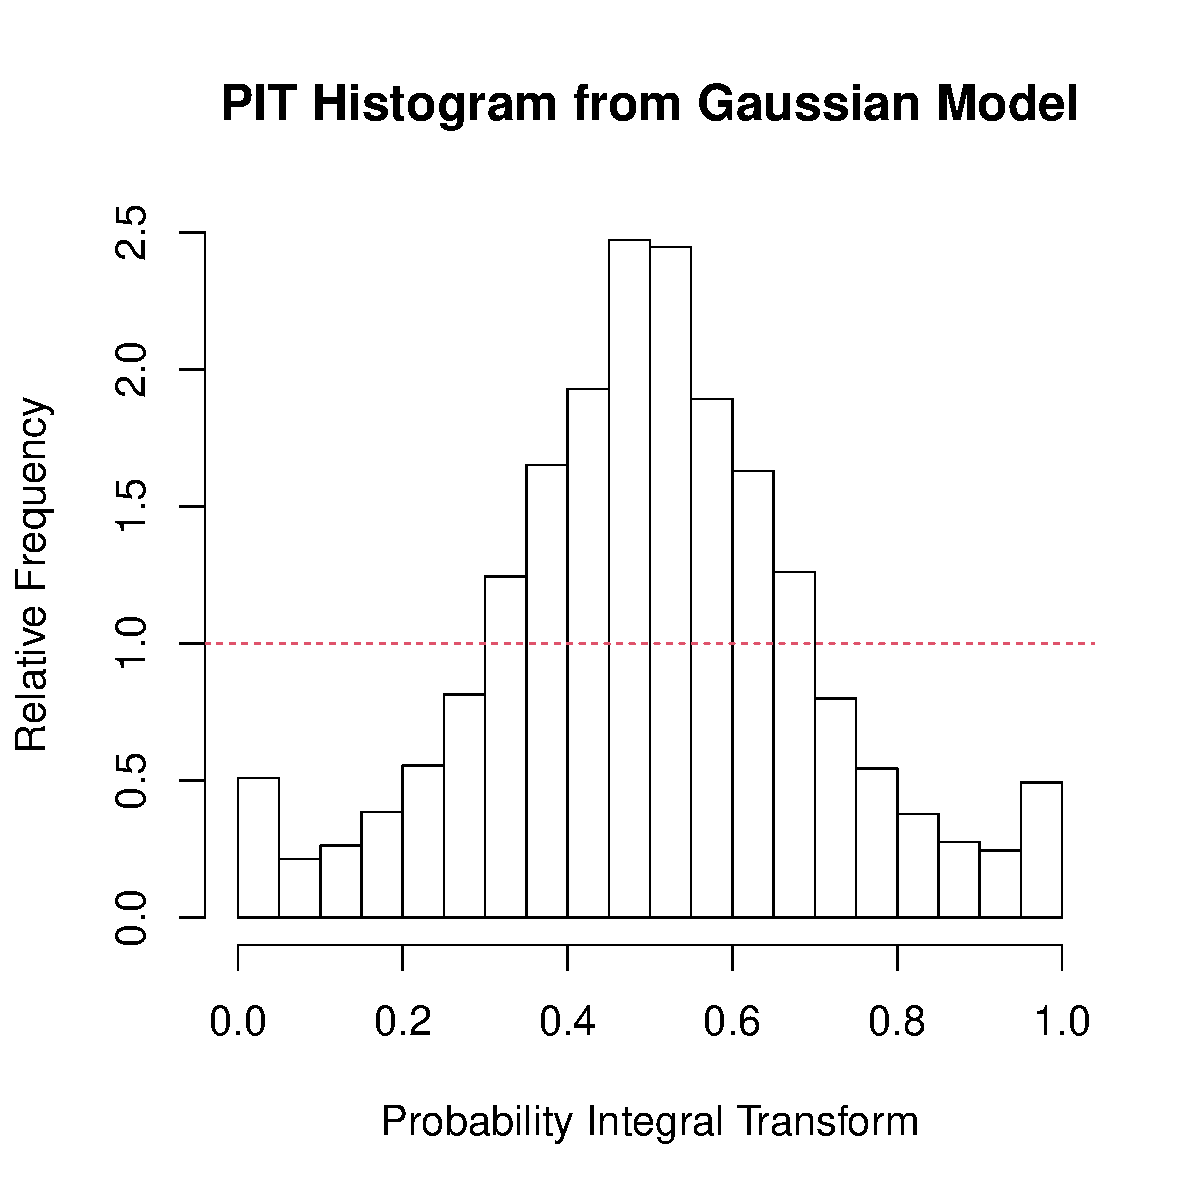
\includegraphics[width=\linewidth]{./figures/PIT_real_Gaussian.pdf}
  \caption{Gaussian Model.}
\end{subfigure}
  \caption{PIT histograms for both TGH and Gaussian model with the real dataset. }
  \label{fig:PIT_real}
\end{figure}


\subsection{TLR/HODLR Matrices Performance Assessment}
We provide the TGH modeling and prediction operations in
low-rank structure using both TLR and HODLR approximations.
The baseline TLR software is the HiCMA library, which runs on
both shared-memory and distributed memory architectures, while
the HODLR underlying software is HODLRLIB, which only has a shared-memory implementation through OpenMP
multithreaded BLAS. We compare the TGH non-Gaussian model using TLR
against HODLR approximations on two
different shared-memory architectures from two vendors, i.e., Intel
and AMD. We assess the performance of both
 implementations of the TGH non-Gaussian likelihood function.


\begin{figure}
\centering
%     \begin{subfigure}[b]{0.38\textwidth}
%     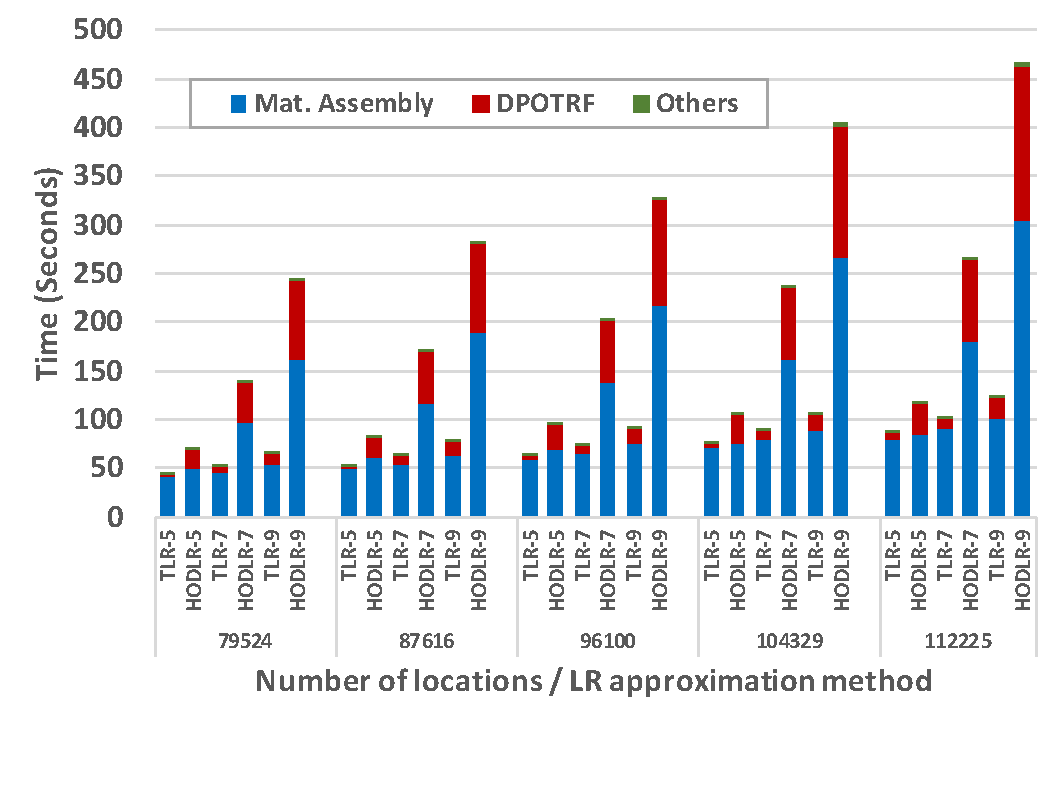
\includegraphics[width=1\textwidth]{./figures/lr-performance-shihab.pdf}
%     \caption{Intel Haswell 36-core}
%      \label{fig:tlrhodlr-shihab}
%    \end{subfigure}
      \begin{subfigure}[b]{0.43\textwidth}
     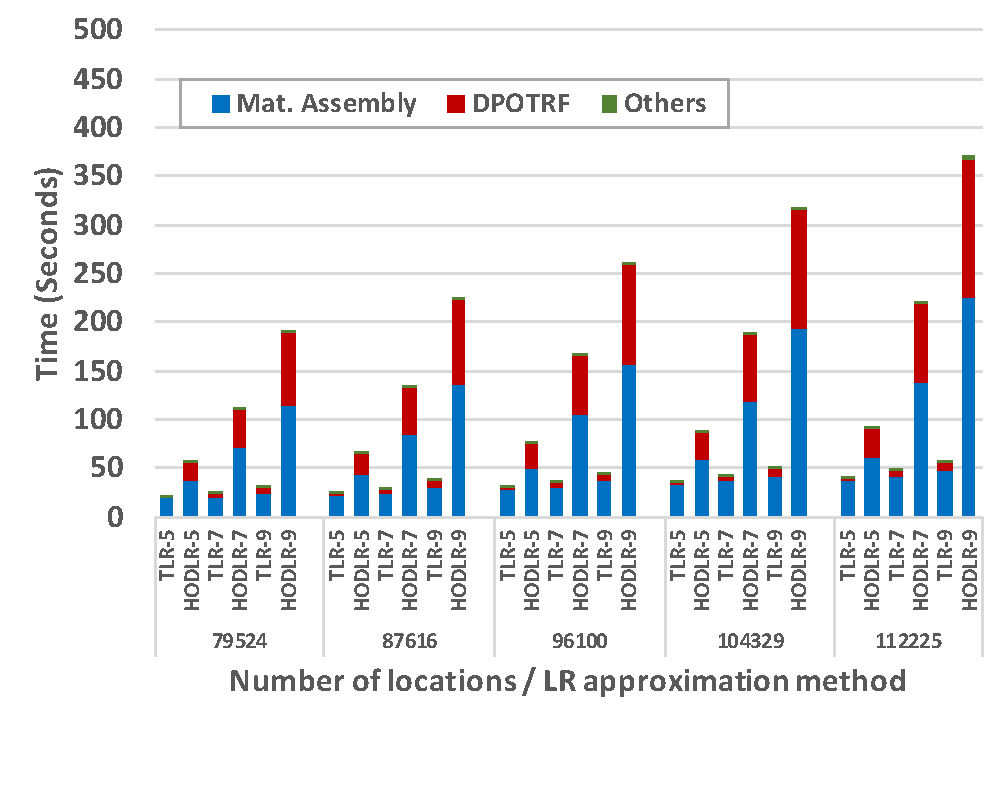
\includegraphics[width=1\textwidth]{./figures/lr-performance-qaysar.pdf}
     \caption{56-core Intel IceLake.}
      \label{fig:tlrhodlr-qaysar}
    \end{subfigure}
     \begin{subfigure}[b]{0.43\textwidth}
     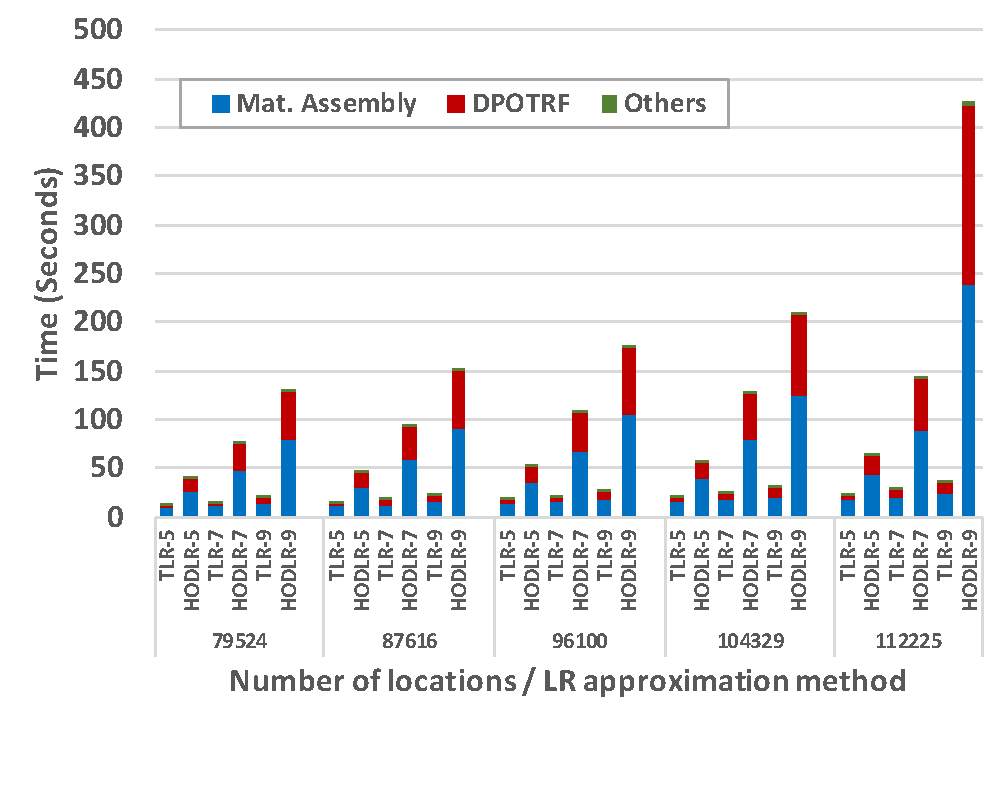
\includegraphics[width=1\textwidth]{./figures/lr-performance-kanary.pdf}
     \caption{128-core AMD Milan.}
     \label{fig:tlrhodlr-kanary}
    \end{subfigure}
%    \begin{subfigure}[b]{0.38\textwidth}
%    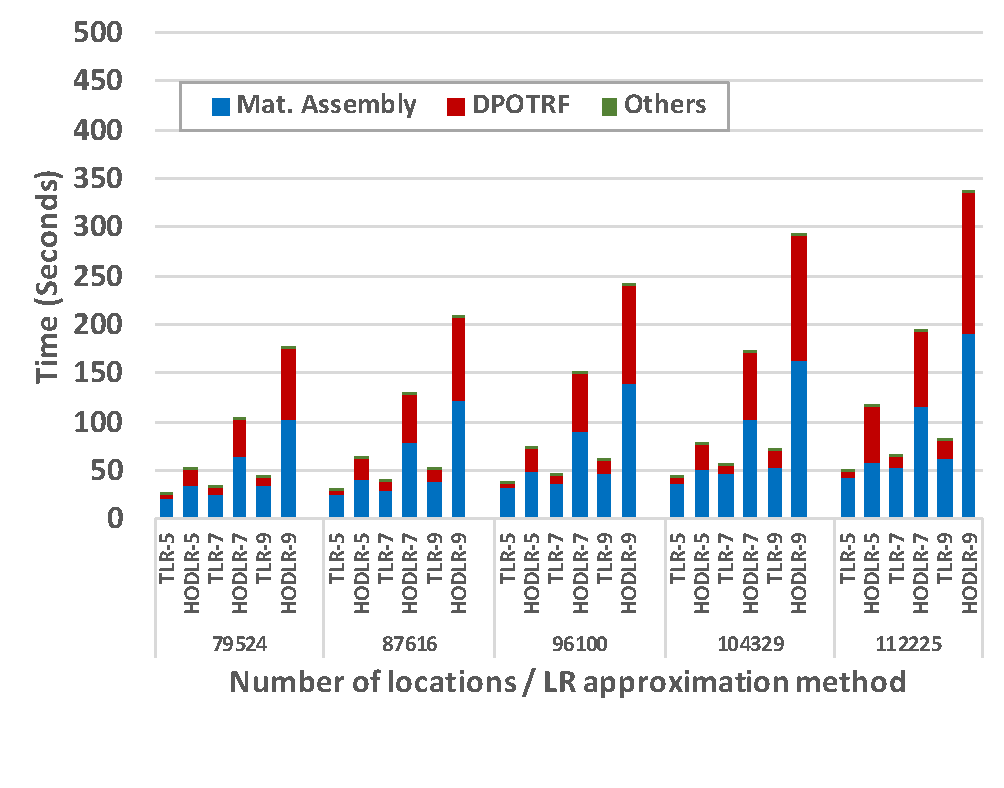
\includegraphics[width=1\textwidth]{./figures/lr-performance-tuwaiq.pdf}
%    \caption{AMD Rome 64-core}
%     \label{fig:tlrhodlr-tuwaiq}
%     \end{subfigure}
     \caption{Time breakdown of a single TGH non-Gaussian likelihood function estimation on two shared-memory systems using TLR and HODLR computations.}
       \label{fig:tlr-vs-hodlr}
     \end{figure}
     
     

Fig.~\ref{fig:tlr-vs-hodlr} shows the breakdown of execution times to
calculate a single TGH likelihood function using both TLR
and HODLR matrices. We report the result of three
accuracy levels for each approximation method using
five dataset sizes. The execution time is broken down into matrix assembly time
(i.e., the time taken to compute the covariance matrix in low-rank structure), matrix factorization time (POTRF), and
others (i.e., matrix determinant computing, measurements vector
transformation, matrix-vector triangular solve (TRSV)).  
The figure highlights that the HiCMA-based
implementation of the TLR approximation is faster than
the HODLRLIB implementation of the HODLR approximation.
Moreover, it can be seen that with different accuracy levels, the total
execution time difference increases between TLR and HODLR. For instance, on Intel IceLake, TLR outperforms HODLR by $2.29X$, $4.66X$, and $6.46X$ with accuracy levels $10^{-5}$, $10^{-7}$, $10^{-9}$, respectively. We also observed that the speedup is strongly influenced by the number of cores; for instance, on AMD Milan, TLR 
outperforms HODLR by $6.82X$ with an accuracy level of $10^{-9}$ which means that HODLRLIB cannot efficiently utilize the 
system resources. This performance difference between HiCMA and HODLRLIB comes mostly
from the programming models: task-based with asynchronous executions (i.e., HiCMA) versus
bulk-synchronous fork-join paradigm (i.e., HODLRLIB).
The figure also shows that assembling the covariance 
matrix with TLR format accounts now for most of the 
likelihood function estimation. The matrix assembly takes up to 
$70\%$ and $85\%$ of the total time on Intel IceLake and AMD Milan, respectively. 
In contrast, due to a slower HODLRLIB MLE, 
the matrix assembly takes about $65\%$ of the total execution time on 
both machines. 



\subsection{TLR Matrices Performance Assessment}
In this section, we compare the performance of TLR 
against exact when computing the non-Gaussian modeling and the prediction operations
on shared and distributed-memory architectures. 



\textbf{Performance on Shared-Memory Systems}
Fig.~\ref{fig:tlr-exact} shows the performance of the
TLR approximation compared to the exact implementation
of the TGH non-Gaussian likelihood function on our target two
shared-memory systems and using different data sizes.  With different accuracy, TLR outperforms the exact version of the likelihood estimation with a different number of locations. TLR shows better performance than the exact implementation, reaching up to $7.29X$ and $5.74X$ on Intel IceLake and AMD Milan, respectively.   Furthermore, Figure~\ref{fig:tlr-exact-pred} shows the performance of the prediction operation using
exact and TLR. The figure shows the TLR approximation of
accuracy $10^{-9}$ outperforms the exact computation with
up to $4.29X$ and $4.88X$ on the given machines.



\begin{figure}
\centering
      \begin{subfigure}[b]{0.33\textwidth}
     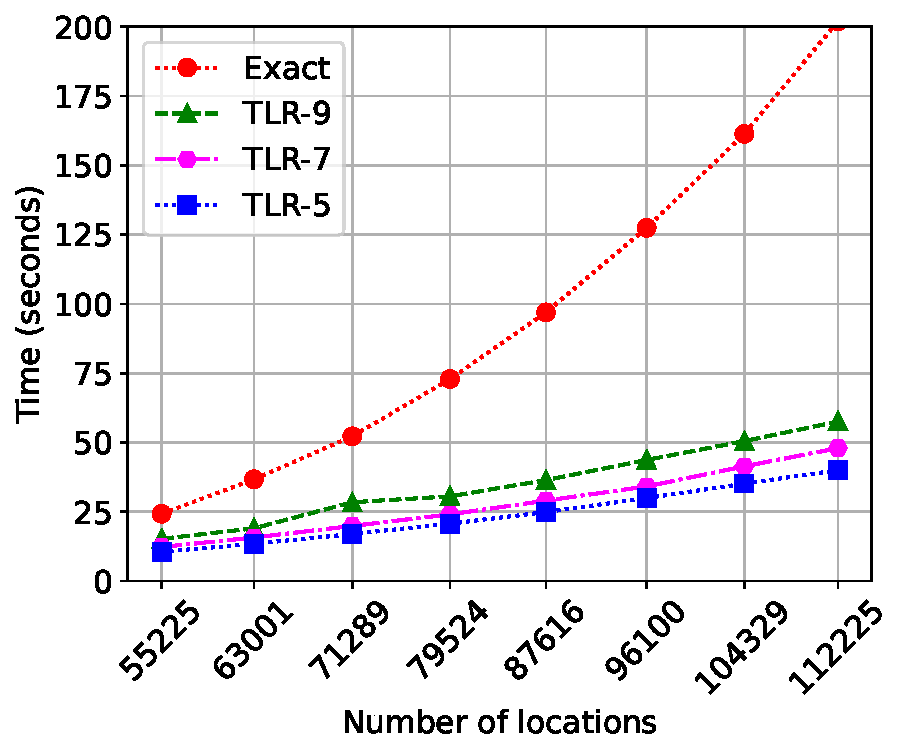
\includegraphics[width=1\textwidth]{./figures/iceLake-56-core-performance.pdf}
     \caption{56-core Intel IceLake.}
      \label{fig:intel-icelake}
    \end{subfigure}
     \begin{subfigure}[b]{0.33\textwidth}
     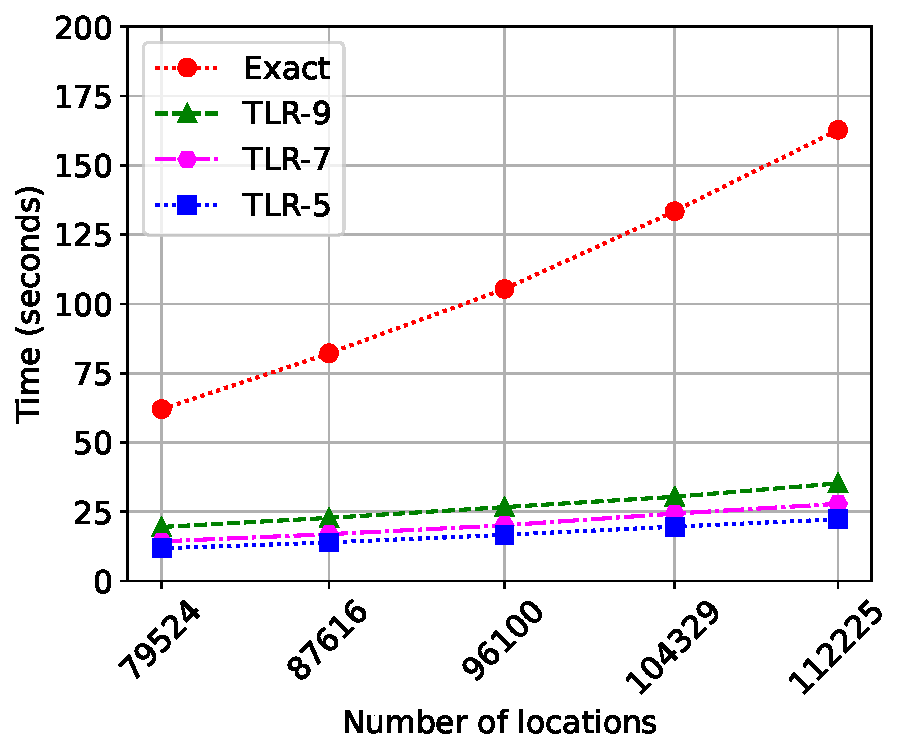
\includegraphics[width=1\textwidth]{./figures/amd-milan-128-core-performance.pdf}
     \caption{128-core AMD Milan.}
     \label{fig:amd-milan}
    \end{subfigure}
%    \begin{subfigure}[b]{0.23\textwidth}
%    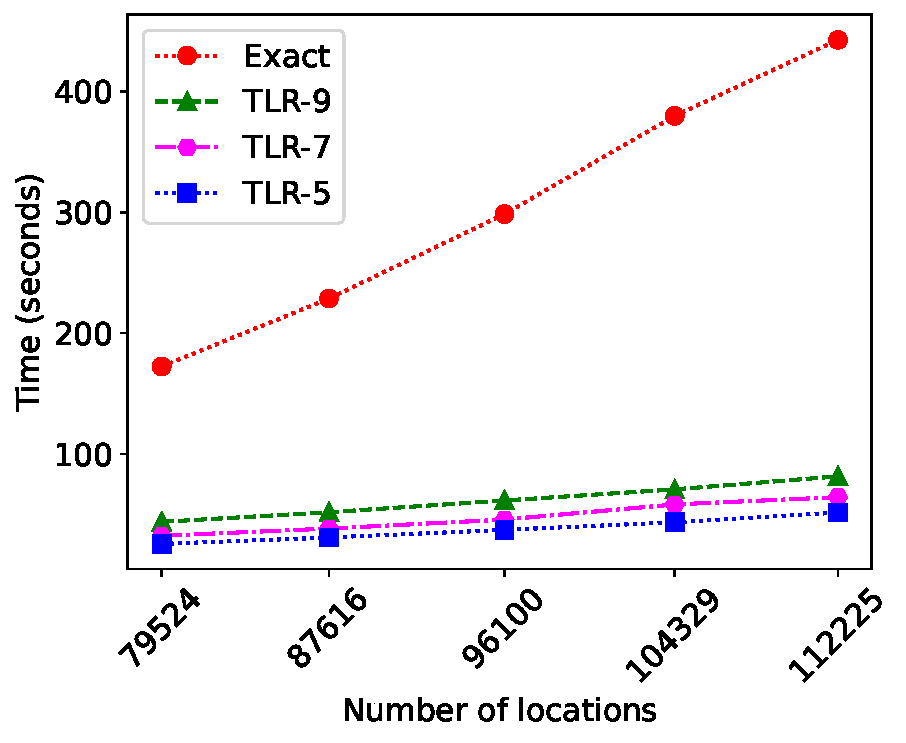
\includegraphics[width=1\textwidth]{./figures/amd-naples-64-core-performance.pdf}
%    \caption{AMD Rome 64-core}
%     \label{fig:amd-rome}
%         \end{subfigure}
%     \begin{subfigure}[b]{0.23\textwidth}
%     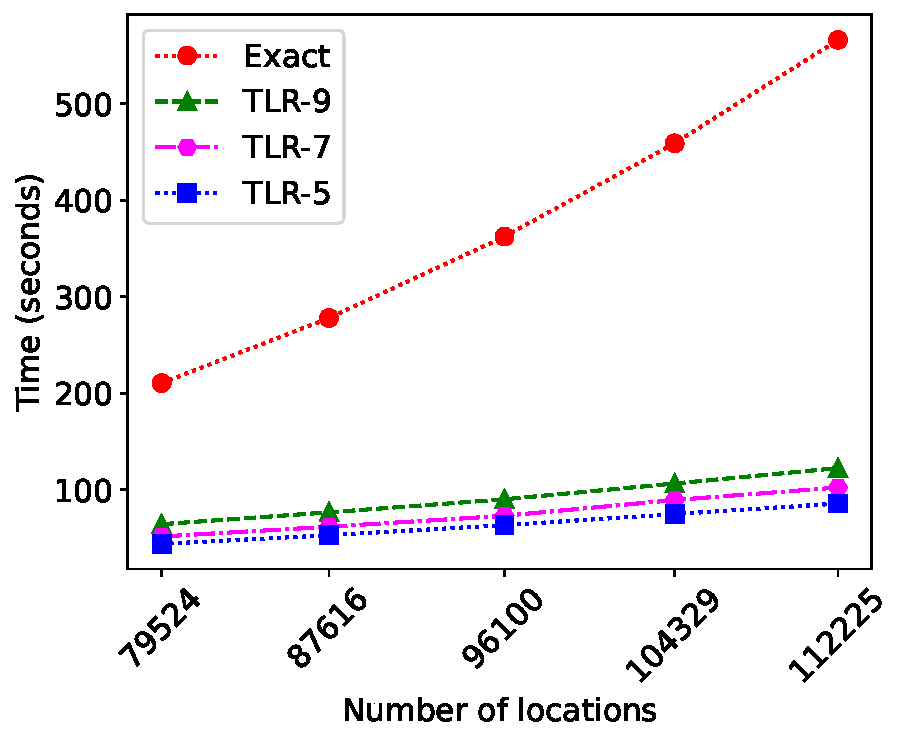
\includegraphics[width=1\textwidth]{./figures/haswell-36-core-performance.pdf}
%     \caption{Intel Haswell 36-core}
%      \label{fig:intel-haswell}
%    \end{subfigure}

     \caption{Performance of a single non-Gaussian MLE iteration on two shared-memory hardware architectures using exact and TLR matrices.}
         \label{fig:tlr-exact}
\end{figure}

\begin{figure}
\centering
      \begin{subfigure}[b]{0.33\textwidth}
     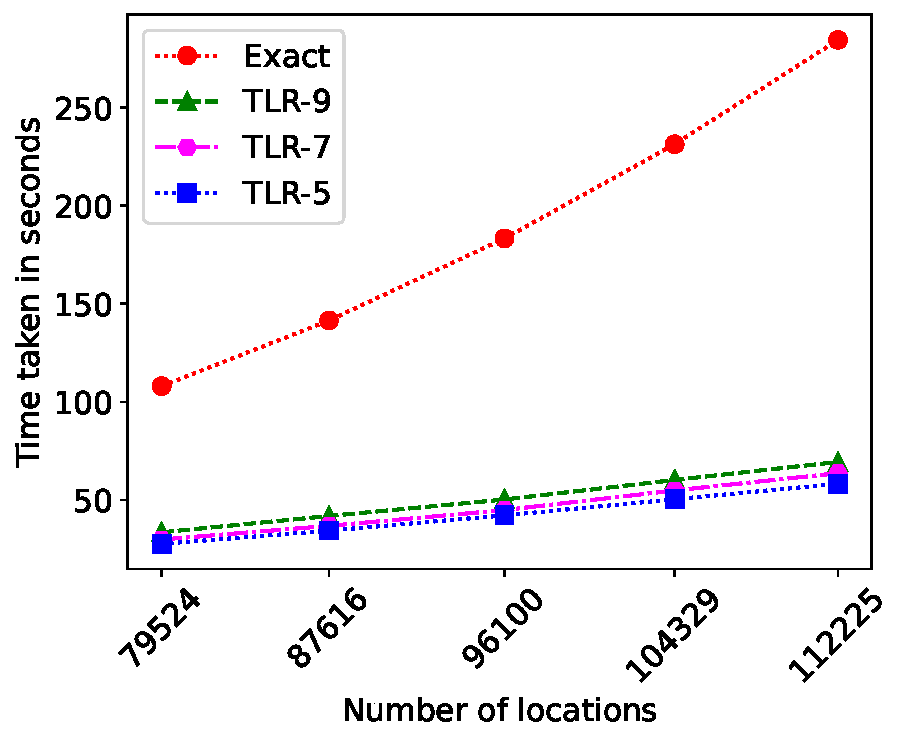
\includegraphics[width=1\textwidth]{./figures/iceLake-56-core-pred-performance.pdf}
     \caption{56-core Intel IceLake.}
      \label{fig:intel-icelake-tlr}
    \end{subfigure}
     \begin{subfigure}[b]{0.33\textwidth}
     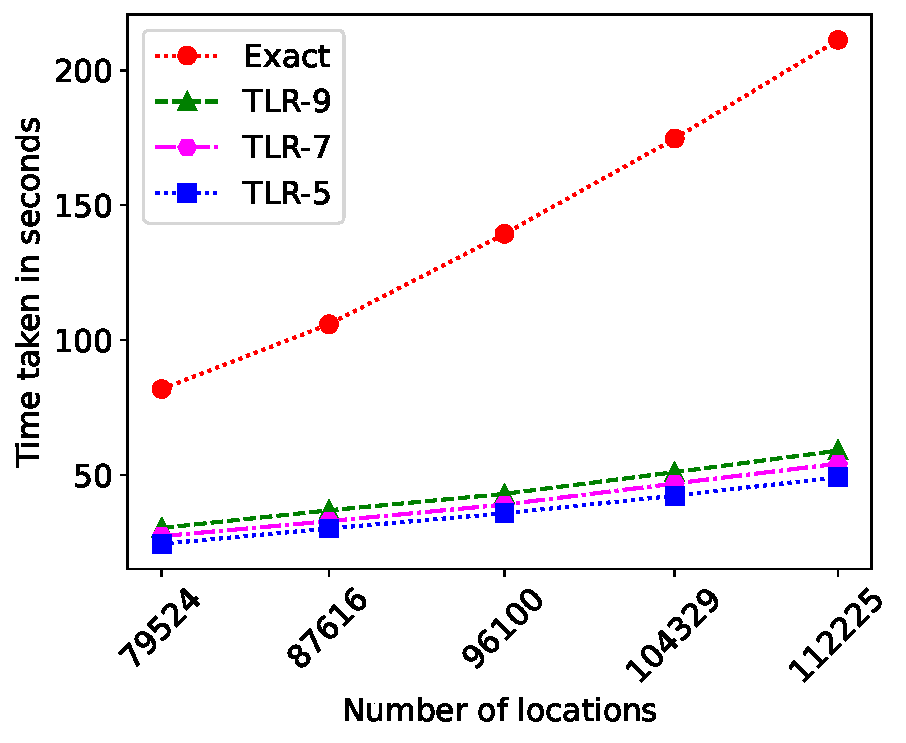
\includegraphics[width=1\textwidth]{./figures/amd-milan-128-core-pred-performance.pdf}
     \caption{128-core AMD Milan.}
     \label{fig:amd-milan-tlr}
    \end{subfigure}
%    \begin{subfigure}[b]{0.23\textwidth}
%    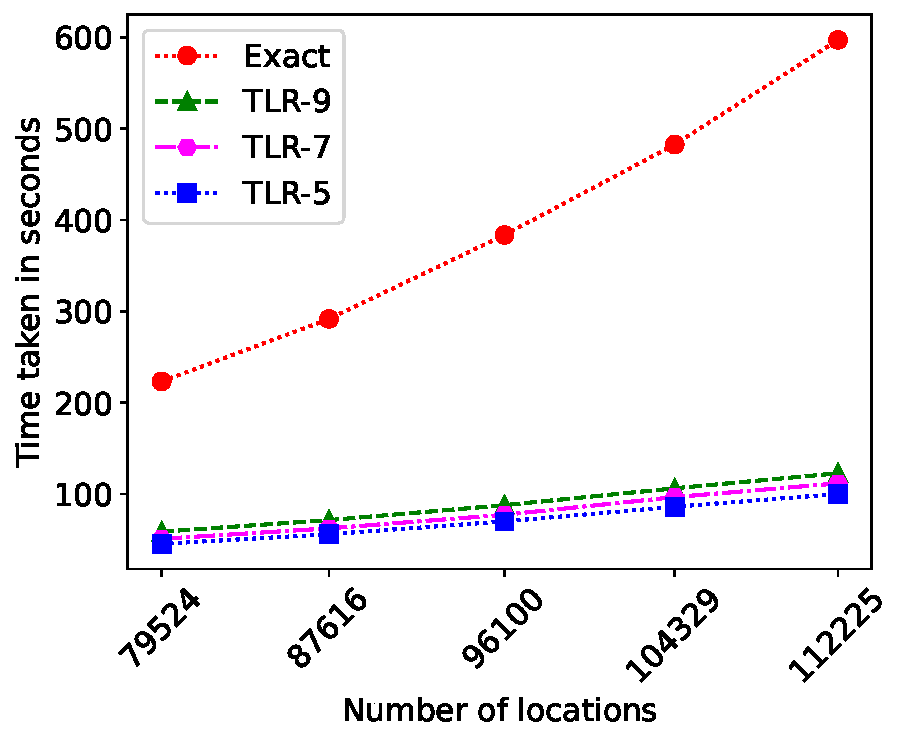
\includegraphics[width=1\textwidth]{./figures/amd-naples-64-core-pred-performance.pdf}
%    \caption{AMD Rome 64-core}
%     \label{fig:amd-rome-tlr}
%         \end{subfigure}
%     \begin{subfigure}[b]{0.23\textwidth}
%     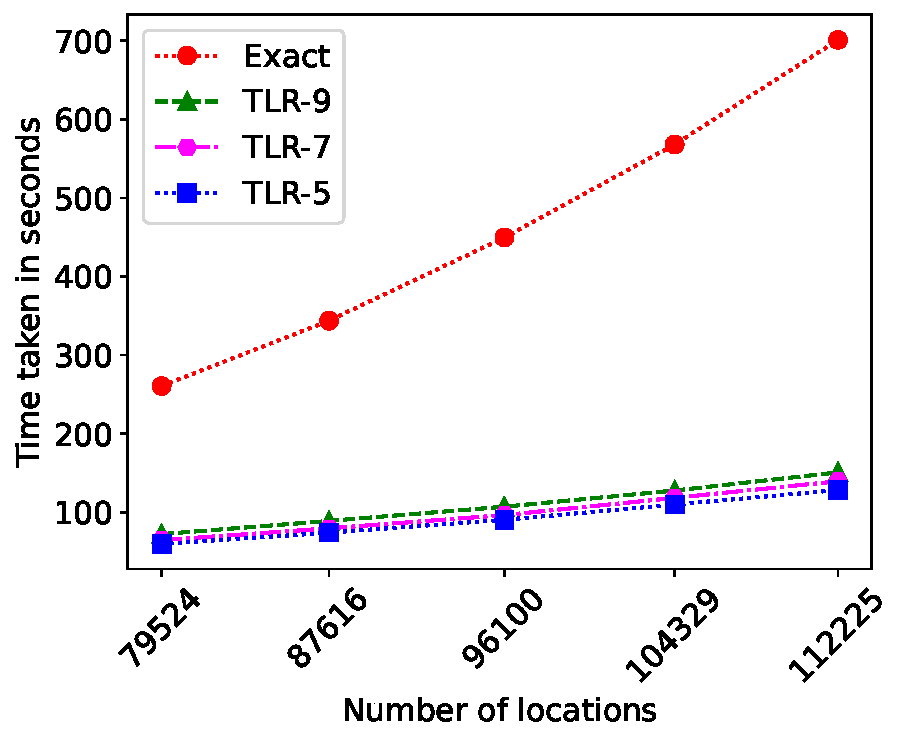
\includegraphics[width=1\textwidth]{./figures/haswell-36-core-pred-performance.pdf}
%     \caption{Intel Haswell 36-core}
%      \label{fig:intel-haswell-tlr}
%    \end{subfigure}

     \caption{Performance of a single TGH non-Gaussian prediction operation on different shared-memory hardware architectures using exact and TLR matrices.}
         \label{fig:tlr-exact-pred}
\end{figure}

\textbf{Performance on Distributed-Memory Systems}
We also assess the performance of the TLR-based approximation
on 512 nodes of a Cray XC40 system. Fig.~\ref{fig:crayxc40} shows
the execution time of the exact and TLR approximation for MLE with different accuracy levels. As shown, the TLR 
approximation shows better performance compared to exact computation with a different number of
 locations up to 800K locations. The figure shows
 that the TLR-approximation outperforms the exact computation with up to $2.96X$.
 We believe the performance of TLR MLE can be further improved by using a runtime
 system that provides rank-aware data distribution to mitigate the load imbalance~\cite{abdulah2021accelerating}.
 % The reported performance is for a tuned tile size and an average of three runs.
  


\begin{figure}[h]
\centering
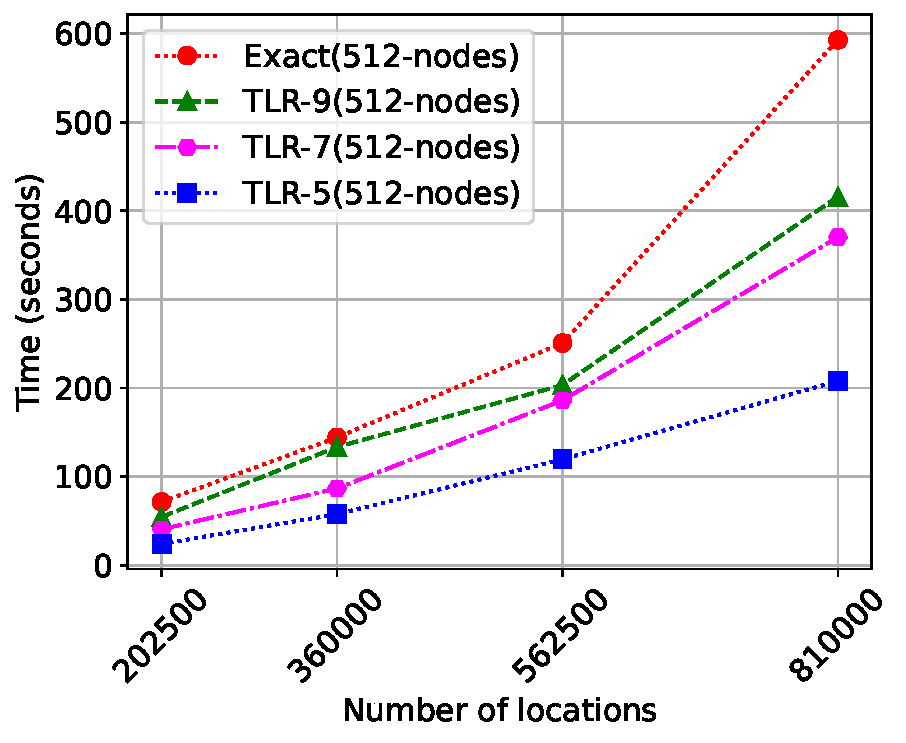
\includegraphics[width=0.75\linewidth]{./figures/shaheen-performance.pdf}
  \caption{Performance of a single non-Gaussian MLE iteration on
Cray XC40 system up to 512 nodes using exact and TLR matrices.
}
  \label{fig:crayxc40}
\end{figure}

\section{Conclusion}
This paper introduces a parallel non-Gaussian modeling and
prediction implementation based on the Tukey $g$-and-$h$ (TGH)
random fields in the context of climate/weather applications. 
We propose a task-based exact computation for both operations
with the aid of existing dense linear algebra libraries to tackle the underlying matrix operation with large problem sizes. We also
assess low-rank approximations using tile low-rank (TLR) and hierarchically
off-diagonal low-rank (HODLR). We rely on HiCMA and HODLRLIB to perform the required
matrix operations for MLE. The TLR approximation carried out
 for  modeling and the prediction
operations outperforms its HODLR counterpart. Using up to $800K$ geospatial locations, it also shows a speedup up to 
$7.29X$ and $2.96X$ compared to the exact implementation on shared and distributed-memory systems,
respectively. For future work, we would like to consider mixed precision arithmetics with GPU
hardware accelerators to boost the performance of dense linear algebra kernels. We would like 
also to investigate randomized algorithms to directly generate the compressed matrix and improve
the matrix assembly phase.
% Furthermore, the TLR implementation
% outperforms the exact implementation by up to  on distributed-memory systems using 800K geospatial locations.


%\begin{thebibliography}{00}

\bibliography{report_bib}

\bibliographystyle{IEEEtran}
\end{document}
